\documentclass[UTF8,a4paper,11pt,fontset=none]{ctexart}

\usepackage[a4paper,top=2.3cm,bottom=2.3cm,left=2.4cm,right=2.4cm]{geometry}
\usepackage{amsmath,amssymb,mathtools}
\usepackage{booktabs,longtable,array,tabularx,multirow}
\usepackage{graphicx,float,placeins}
\usepackage{xcolor}
\usepackage{enumitem}
\usepackage{listings}
\usepackage{caption}
\usepackage[hidelinks]{hyperref}
\usepackage{setspace}

\ctexset{
  section={format=\zihao{3}\bfseries\centering,beforeskip=1.2ex,afterskip=0.8ex},
  subsection={format=\zihao{4}\bfseries,beforeskip=0.9ex,afterskip=0.5ex}
}
\setmainfont{Times New Roman}
\setCJKmainfont[AutoFakeBold=2.5]{SimSun}
\setCJKsansfont{SimHei}
\setCJKmonofont{FangSong}
\setstretch{1.18}
\setlength{\parindent}{2em}
\setlength{\parskip}{0pt}
\setlength{\emergencystretch}{2em}
\Urlmuskip=0mu plus 1mu
\setlength{\LTpre}{0.4em}
\setlength{\LTpost}{0.4em}
\renewcommand{\arraystretch}{1.12}
\graphicspath{{generated/figures/}}
\pagestyle{plain}
\setcounter{secnumdepth}{2}
\setcounter{tocdepth}{2}

\captionsetup{font=small,labelfont=bf,labelsep=space}
\hypersetup{
  pdftitle={信息时序约束下的世界杯收视预测、赛程协同与动态资源优化},
  pdfauthor={},
  pdfsubject={2026年度策联杯数学建模精英联赛C题}
}

\definecolor{codegray}{RGB}{70,70,70}
\definecolor{codebg}{RGB}{248,248,248}
\lstset{
  basicstyle=\ttfamily\scriptsize,
  keywordstyle=\color{blue!60!black},
  commentstyle=\color{green!40!black},
  stringstyle=\color{red!55!black},
  backgroundcolor=\color{codebg},
  frame=single,
  breaklines=true,
  breakatwhitespace=false,
  showstringspaces=false,
  numbers=left,
  numberstyle=\tiny\color{codegray},
  numbersep=6pt,
  tabsize=4,
  columns=fullflexible,
  keepspaces=true
}

\providecommand{\tightlist}{%
  \setlength{\itemsep}{0pt}\setlength{\parskip}{0pt}}

\begin{document}
\pagenumbering{arabic}
\setcounter{page}{1}

\begin{center}
  {\zihao{2}\bfseries 信息时序约束下的世界杯收视预测、赛程协同与动态资源优化\par}
\end{center}
\vspace{0.8em}

\begin{center}
  {\zihao{3}\bfseries 摘\quad 要}
\end{center}

针对大型足球赛事中收视预测、赛程安排、动态资源配置和实际赛程评价相互依赖的问题，本文建立遵守信息时点的顺序决策链。首先，仅使用赛前可得信息构造交换球队顺序后不变的对称特征，并在统一特征函数中规范化赛事名称。扩窗时间验证显示，Elastic Net 的 MSE、RMSE 和 MAE 分别为 188.9787、13.7268 和 10.6345，优于均值基线和 Extra Trees；规范化后 72 场未来比赛的未见赛事类别计数为 0。其次，将 72 场收视预测输入时段 MILP 和固定时段后的场馆 MILP，得到综合目标值 0.272453；所有球队均获得 2 场黄金时段和 1 场大容量场馆比赛，同组相邻轮次最小间隔为 63 小时。再次，固定第三轮赛程，在第三轮开始前的统一信息截面上同时模拟 24 场比赛 20000 次，对完全同分情形分配等比例晋级权重。动态总净值为 6.583849，较静态方案的 6.578368 提高 0.083318\%；五个随机种子下的改善率位于 0.080406\% 至 0.084923\%，说明该边际改善对 Monte Carlo 随机种子稳定。最后，以 2022 年世界杯为参照，分层比较直接结构事实、映射辅助指标和完整题内代理指标。最近邻和第二近邻映射下实际赛程代理综合值分别为 0.196995 和 0.210331，均低于优化赛程的 0.272453，但举办区域尺度和赛事规模会显著影响旅行、休息与场馆利用等结构指标，代理综合值不能替代对真实赛事的全面评价。

\vspace{0.8em}
\noindent\textbf{关键词：}收视预测；混合整数规划；联合泊松模拟；动态资源配置；赛程评价

\newpage

\section{问题重述}

赛事组织者需要在比赛尚未开始时估计转播需求，据此安排 72 场小组赛的场馆和开球时段；当前两轮结束后，部分球队的晋级形势、市场反馈和风险水平发生变化，又需要在保持第三轮赛程不变的前提下调整转播、安保、交通和票价。赛后还需将优化方案置于真实赛事背景中评价，判断收益、公平和执行代价之间的取舍。

四个问题并非彼此独立。问题一产生的 72 场转播观看人数预测进入问题二的转播价值；问题二产生的第三轮场馆与时段是问题三的固定输入；问题四则沿用问题二的指标定义和权重。若混淆信息时点，例如用测试标签更新后续测试特征，或让某场第三轮结果影响另一场第三轮比赛，就会使方案获得现实中不可用的信息优势。因此，本文将信息可得性与硬约束同时纳入建模。

\begin{figure}[htbp]
\centering
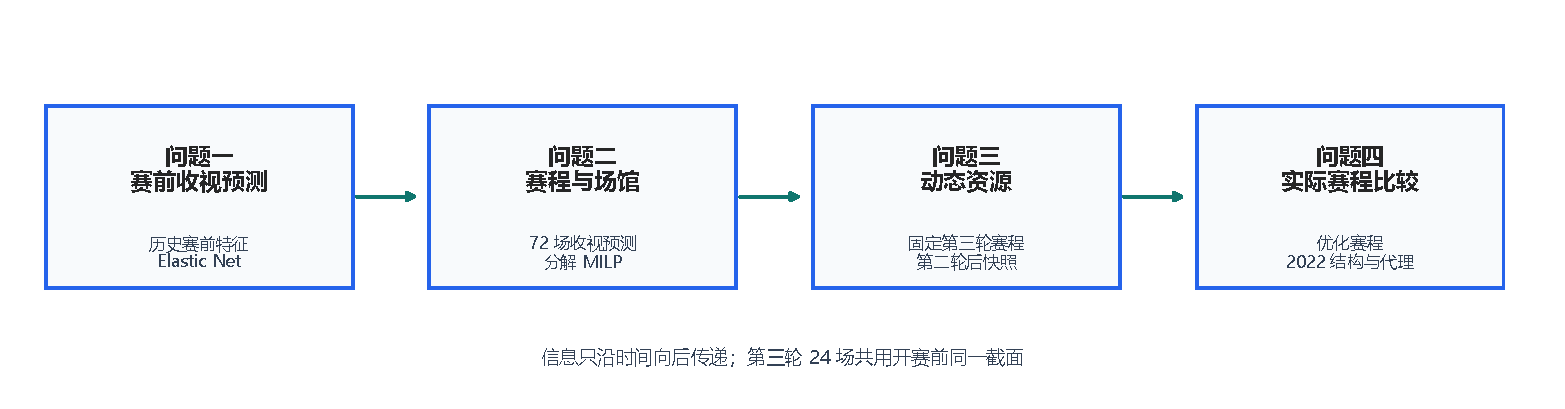
\includegraphics[width=0.98\textwidth]{fig_information_flow.pdf}
\caption{四问顺序决策与信息流。箭头表示计算输出的传递，不表示允许使用未来信息。}
\label{fig:information-flow}
\end{figure}

图~\ref{fig:information-flow} 给出全文证据链：问题一输出进入问题二的转播价值，问题二固定第三轮时空安排，问题三只在该安排上重新分配资源，问题四再将优化结果放回实际赛事中比较。

\section{数据、假设与符号}

\subsection{数据及信息时点}

题目附件提供历史比赛、球队属性、72 场对阵及赛前预测、场馆、时段、距离矩阵、安保要求、动态资源限制和前两轮反馈\cite{problem2026}。问题四另使用固定版本的 2022 年世界杯赛程、赛前 Elo 和实体映射。各阶段允许使用的信息见表~\ref{tab:information-timing}。

\begin{longtable}[]{@{}>{\raggedright\arraybackslash}p{0.16\textwidth}p{0.37\textwidth}p{0.37\textwidth}@{}}
\caption{信息时点与禁用信息}\label{tab:information-timing}\\
\toprule\noalign{}
阶段 & 可用信息 & 禁用信息 \\
\midrule\noalign{}
\endhead
\bottomrule\noalign{}
\endlastfoot
问题一训练 & 历史比赛的赛前字段及训练标签 & 同场进球、射门、控球、实际上座等赛后字段作为特征 \\
问题一测试与 72 场预测 & 统一赛前特征 & 测试标签、同场赛果和实际观众 \\
问题二 & 问题一预测、72 场赛前参数、场馆与时段信息 & 前两轮真实赛果 \\
问题三静态方案 & 赛前预计观众、预计收视、吸引力和赛前风险 & 前两轮更新后的晋级概率和风险 \\
问题三动态方案 & 前两轮结束后的统一信息截面 & 任一第三轮比赛结果 \\
问题四 & 2022 年赛程事实、赛前 Elo 和题内映射参数 & 无来源的真实商业、票务或安保参数 \\
\end{longtable}

所有时间先转换为 UTC 计算冲突和休息约束，再按场馆时区计算当地日期。问题一测试输出单位为百万人，72 场预测输出单位为人。问题二和问题三的货币量按题目字段分别使用美元或百万美元，表格中均注明口径。随机过程采用固定种子：问题一随机模型、问题三主模拟与模拟次数检查均为 20260816，问题三五种子为 20260816--20260820，问题四 2000 组权重扰动为 20260816。

\subsection{基本假设}

\begin{enumerate}
\def\labelenumi{\arabic{enumi}.}
\tightlist
\item
  附件中标注为赛前参数的评分和概率在相应决策时点可获得。
\item
  第三轮 24 场共享第三轮开始前的同一信息截面；给定更新状态后，各场进球数按题面泊松模型生成。
\item
  场馆容量、安保能力、资源上限和成本系数在研究期内不变。
\item
  题目给定的候选时段、资源等级和价格边界构成完整可行动作集合。
\item
  问题四无法直接观测的商业与风险指标仅通过题内映射估计，不视为 2022 年真实经营数据。
\end{enumerate}

\subsection{主要符号}

主要符号见表~\ref{tab:symbols}。

\begin{longtable}[]{@{}ll@{}}
\caption{主要符号及含义}\label{tab:symbols}\\
\toprule\noalign{}
符号 & 含义 \\
\midrule\noalign{}
\endhead
\bottomrule\noalign{}
\endlastfoot
\texttt{i、t、v、s} & 比赛、球队、场馆、时段索引 \\
\texttt{x\_is} & 比赛 \texttt{i} 是否选择时段 \texttt{s} \\
\texttt{z\_iv} & 比赛 \texttt{i} 是否选择场馆 \texttt{v} \\
\texttt{V\_hat\_i} & 问题一预测的转播观看人数 \\
\texttt{T、B、U、H} & 票务、转播、悬念、吸引力指标 \\
\texttt{C、D、F、R} & 成本、旅行、公平、风险指标 \\
\texttt{S\_t、h\_t} & 前两轮后的球队状态和伤病影响 \\
\texttt{p\_t} & 球队晋级概率 \\
\texttt{delta\_i} & 第三轮比赛票价调整比例 \\
\texttt{Z\_2、Z\_3} & 问题二和问题三综合目标 \\
\end{longtable}

\section{转播观看人数预测}

\subsection{建模思路}

历史数据只有 560 个训练样本，而特征包含连续变量和类别变量；测试集又处于训练时间之后。随机划分会把较晚比赛的信息混入训练，因此本文按日期采用扩窗验证。另一方面，\texttt{team\_a} 和 \texttt{team\_b} 只是记录顺序，并非主客队。若直接保留双方有序类别或带符号差值，交换记录顺序就可能改变预测。为此，本文使用统一的对称特征生成函数，并在测试和 72 场预测中保持完全相同的口径。

\subsection{对称赛前特征}

对排名和 Elo，构造双方的均值、最小值、最大值和绝对差；对市值、平均年龄、明星指数、球迷基础、攻防风格、东道主标记和综合实力采用同样变换。胜平负赔率先转换为归一化赛前概率，保留平局概率、双方胜率的最小值、最大值和绝对差，并构造归一化概率熵：

\[
E_i^{\mathrm{prob}}=-\frac{1}{\log 3}
\sum_{o\in\{W,D,L\}}p_{io}\log p_{io}.
\]

其他特征包括中立场标记、月份、星期、赛事类型和归并后的比赛阶段。赛事名称先经确定性函数清理大小写、年份和 FIFA 前缀，将 \texttt{World Cup}、\texttt{FIFA World Cup} 及带年份的同义写法统一为 \texttt{World Cup}；训练、验证、测试和 72 场预测共用这一函数和类别字典。历史训练集中缺少与未来数据统一生成口径的 \path{expected_attendance_base}、\path{attractiveness_index}、\path{commercial_value_index} 和 \path{uncertainty_index}，故这些字段不进入回归；悬念只由统一的赛前胜平负概率表示。模型也不使用球队有序类别、同场赛果和任何测试期滚动标签。

观看人数具有右偏和量级差异。设原始观看人数 \texttt{y\_i} 的单位为人，训练目标定义为：

\[
q_i=\log\left(1+\frac{y_i}{10^6}\right).
\]

模型预测后通过

\[
\widehat y_i^{\mathrm{million}}=\exp(\widehat q_i)-1
\]

还原为百万人，再按输出模板决定是否乘以一百万。该变换减弱少数大观看量比赛对拟合的支配，同时保持逆变换结果非负。

\subsection{模型与时间验证}

本文比较均值基线、Elastic Net 和 Extra Trees\cite{zou2005,geurts2006}。数值特征先以训练子窗中位数填补并标准化，类别特征用众数填补和独热编码。Elastic Net 的目标为：

\[
\min_{\boldsymbol\beta}
\frac{1}{2n}\left\|\boldsymbol q-X\boldsymbol\beta\right\|_2^2
+\alpha\left[
\rho\left\|\boldsymbol\beta\right\|_1
+\frac{1-\rho}{2}\left\|\boldsymbol\beta\right\|_2^2
\right],
\]

其中程序取 \texttt{alpha=0.02}、\texttt{rho=0.10}。扩窗验证依次使用前 60\%、70\% 和 80\% 的时间有序样本训练，并在紧随其后的时间窗验证。误差均在逆变换后的百万人尺度计算：

\[
\mathrm{MSE}=\frac{1}{n}\sum_{i=1}^{n}(y_i-\widehat y_i)^2,
\]

\[
\mathrm{RMSE}=\sqrt{\mathrm{MSE}},\qquad
\mathrm{MAE}=\frac{1}{n}\sum_{i=1}^{n}|y_i-\widehat y_i|.
\]

\begin{longtable}[]{@{}lrrr@{}}
\caption{三种模型的扩窗验证结果}\label{tab:q1-model-comparison}\\
\toprule\noalign{}
模型 & MSE & RMSE & MAE \\
\midrule\noalign{}
\endhead
\bottomrule\noalign{}
\endlastfoot
Elastic Net & 188.978683 & 13.726811 & 10.634511 \\
Extra Trees & 227.022897 & 15.033564 & 12.094744 \\
均值基线 & 531.378075 & 22.996821 & 18.398928 \\
\end{longtable}

表~\ref{tab:q1-model-comparison} 中每个指标均先在各折独立计算，再对三折作算术平均，因此汇总 RMSE 不等于汇总 MSE 的平方根。Elastic Net 的三项平均误差均最低，因此选择其作为最终模型。选择依据是时间外验证误差与复现稳定性，而不是预设线性模型一定优于树模型。

为检查平均误差是否掩盖时间段波动，表~\ref{tab:q1-folds} 进一步给出 Elastic Net 的三个扩窗。每个验证窗均含 56 场比赛，且严格位于对应训练窗之后。

\begin{table}[htbp]
\centering
\caption{Elastic Net 的三折扩窗验证结果，误差单位为百万人}
\label{tab:q1-folds}
\small
\begin{tabular}{crrccrrr}
\toprule
折 & 训练数 & 验证数 & 训练截止 & 验证区间 & MSE & RMSE & MAE\\
\midrule
1 & 336 & 56 & 2022-01-13 & 2022-01-18--2022-09-22 & 201.0861 & 14.1805 & 11.2902\\
2 & 392 & 56 & 2022-09-22 & 2022-09-24--2023-04-29 & 205.1182 & 14.3219 & 10.9816\\
3 & 448 & 56 & 2023-04-29 & 2023-04-30--2024-01-07 & 160.7317 & 12.6780 & 9.6318\\
\bottomrule
\end{tabular}
\end{table}

前两折 RMSE 只相差 0.1415，第三折下降至 12.6780；因此误差没有随预测时间后移而恶化，但也不能将三折描述为完全不变。MSE 的折间标准差为 24.5456，提示赛事组成和时间窗仍会影响误差。

\subsection{系数、验证预测与残差}

数值特征经标准化，而类别特征为 0--1 独热指示量，因此两类系数不宜作严格的绝对大小排名。图~\ref{fig:q1-diagnostics}(b) 只用于识别方向和特征族：\texttt{World Cup} 指示量系数为 0.128338；球迷基础均值、最小值和最大值分别为 0.049762、0.038872 和 0.014968；综合实力绝对差与市值绝对差分别为 $-0.018812$ 和 $-0.009680$。由于均值、最小、最大和绝对差之间存在线性关联，本文只解释“球迷基础整体正向”、“实力和市值差异整体负向”，不把任一单列系数解释为独立因果效应。

\begin{figure}[htbp]
\centering
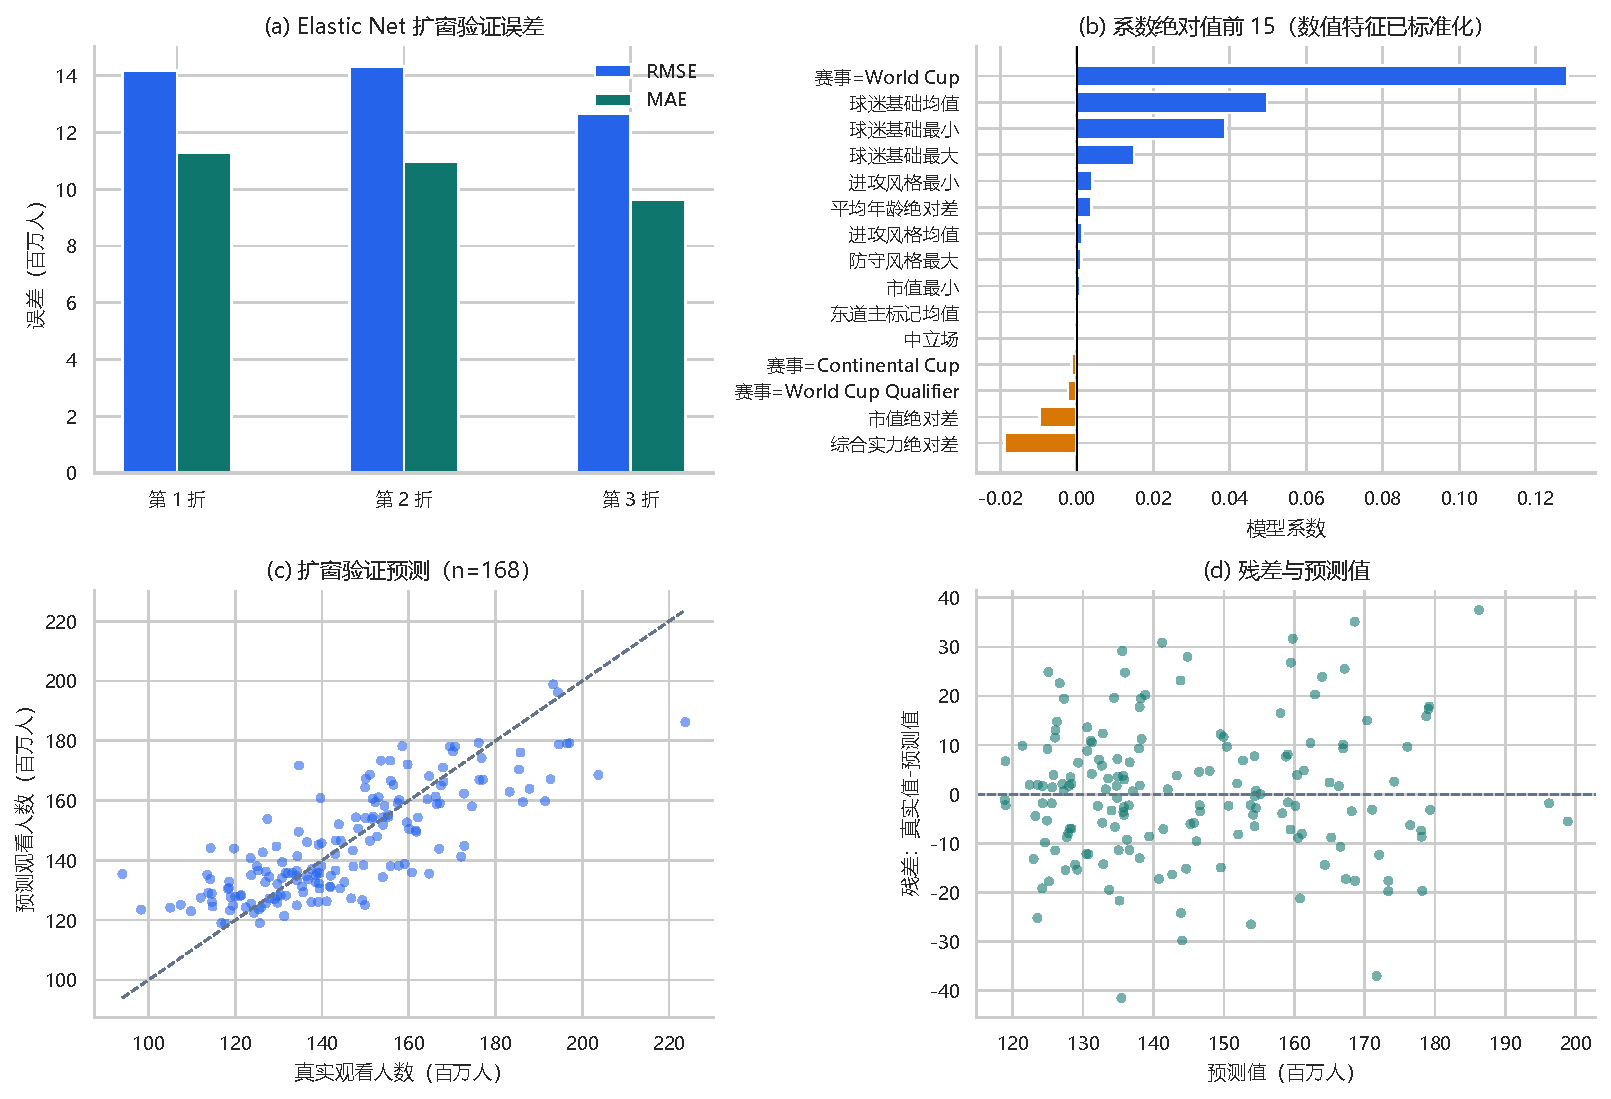
\includegraphics[width=0.98\textwidth]{fig_q1_validation_coefficients_residuals.pdf}
\caption{问题一的扩窗误差、模型系数和验证残差。散点只使用 168 个训练集内时间验证样本，不使用隐藏测试标签。}
\label{fig:q1-diagnostics}
\end{figure}

图~\ref{fig:q1-diagnostics}(c) 显示预测与真实值保持明显正关联，168 个时间外验证样本的相关系数为 0.801153，平均残差（真实值减预测值）为 0.292706 百万人。但最低真实值十分位平均被高估 16.852850 百万人，最高十分位平均被低估 17.624260 百万人。这是对数目标、线性收缩和 Elastic Net 惩罚共同导致的“向中心收缩”：它提高时间外稳定性，但牺牲对极端热门或冷门比赛的幅度拟合。因此后续排程中更适合将该预测视为统一口径下的相对转播需求，而非极端场次的无偏点预测。

\subsection{预测结果与解释}

训练集拟合、测试集预测和 72 场预测的分布见表~\ref{tab:q1-distribution}。

\begin{longtable}[]{@{}lrrrr@{}}
\caption{问题一预测分布，单位：百万人}\label{tab:q1-distribution}\\
\toprule\noalign{}
数据 & 均值 & 标准差 & 最小值 & 最大值 \\
\midrule\noalign{}
\endhead
\bottomrule\noalign{}
\endlastfoot
训练集拟合 & 144.811868 & 17.522965 & 114.222923 & 201.907400 \\
测试集预测 & 144.558531 & 15.800763 & 114.044606 & 180.352371 \\
72 场预测 & 161.599758 & 16.777979 & 134.524563 & 204.108108 \\
\end{longtable}

未来 72 场均值比训练集拟合均值高 16.787890 百万人，约为 11.59\%。对线性预测器的均值变化分解显示，未来样本全部处于世界杯类别，\texttt{World Cup} 指示量对对数预测的平均贡献为 0.120546，是均值上升的主要来源。综合实力绝对差、球迷基础最小值和市值绝对差分别贡献 $-0.005131$、$-0.003977$ 和 $-0.001919$，部分抵消了赛事类别的正向作用。这说明未来预测的提高主要来自世界杯赛事层级，而强弱分明且较弱一方球迷基础偏低的小组赛组合会拉低具体场次的预测。

规范化前，72 场默认赛事名称为 \texttt{FIFA World Cup}；规范化后均为训练集已见的 \texttt{World Cup}，测试集和未来 72 场的未见赛事类别样本数均为 0。该处理位于统一特征函数，而非对未来 CSV 的事后修正。其他连续特征均未超出训练均值正负 4 个标准差。

交换每场双方及对应赛前字段后，最大预测差为 0，证明记录顺序不会影响结果。最终文件包含 140 条测试预测和 72 条小组赛预测，ID 与模板逐项一致，数值均有限且非负。

\FloatBarrier

\section{场馆与开球时段协同优化}

\subsection{指标与变量}

问题二需要在 80 个候选时段和 16 个场馆中安排 72 场比赛。为与实际分解求解一致，定义：

\[
x_{is}=\begin{cases}
1,&\text{比赛 }i\text{ 选择时段 }s,\\
0,&\text{否则},
\end{cases}
\]

\[
z_{iv}=\begin{cases}
1,&\text{比赛 }i\text{ 选择场馆 }v,\\
0,&\text{否则}.
\end{cases}
\]

场馆启用变量记作 \texttt{y\_v}。由于每个场馆的最小承办场次均大于 0，本数据中全部 \texttt{y\_v=1}，启用成本对所有可行方案相同，不作为实际自由决策变量。

比赛 \texttt{i} 在场馆 \texttt{v} 的预计观众和票务价值为：

\[
N_{iv}=\min(N_i^{\mathrm{base}},K_v),
\]

\[
T_{iv}=P_i^{\mathrm{base}}N_{iv}.
\]

问题一输出进入时段转播价值：

\[
B_{is}=\widehat V_i u_i^{\mathrm{broadcast}}
g_s^{\mathrm{prime}}w_i^{\mathrm{sponsor}}.
\]

赛事组织成本以百万美元计：

\[
C=\sum_v c_v^{\mathrm{setup}}y_v+
\sum_{i,v}z_{iv}\left(
c_v^{\mathrm{operation}}+0.1L_i^{\mathrm{req}}c_v^{\mathrm{security}}
\right).
\]

执行风险为：

\[
R_{iv}=0.5r_v^{\mathrm{climate}}
+0.3\frac{N_{iv}}{K_v}
+0.2\frac{L_i^{\mathrm{req}}}{L_v^{\mathrm{security}}}.
\]

悬念 $U$ 直接取附件 \path{uncertainty_index} 的赛程平均，吸引力 $H$ 取 \path{attractiveness_index}/100 的赛程平均。由于 72 场对阵固定，二者在排程优化中是常数项，但仍按题目权重进入最终综合评价。

\subsection{旅行负担代理与公平性}

距离、旅行时间和时区差先分别在全部合法比赛-场馆候选上作 Min-Max 标准化，再合成：

\[
D_{iv}=0.5d_{iv}^{\mathrm{km}}
+0.3d_{iv}^{\mathrm{time}}
+0.2d_{iv}^{\mathrm{tz}}.
\]

第一轮使用球队代表地至当前候选场馆的三个分项；第二、三轮使用该队上一轮全部安保合格候选场馆至当前候选场馆的分项均值；一场比赛再对两队取平均。因此 \texttt{D\_iv} 是候选前序场馆下的期望旅行负担代理，不是最终排程中上一轮实际场馆至当前场馆的真实路线。该定义与题面候选口径一致，也使场馆选择能够在固定时段后独立求解，但没有通过场馆转移变量完全耦合相邻轮次。

黄金时段由 \texttt{global\_prime\_score} 降序、\texttt{slot\_id} 升序稳定处理并列后严格选取前 20 个；大容量场馆为容量前 4 名。设球队黄金时段次数和大容量场馆次数的极差分别为 \texttt{Delta\_prime} 与 \texttt{Delta\_large}，公平性为：

\[
F=\frac{\Delta_{\mathrm{prime}}+\Delta_{\mathrm{large}}}{6}.
\]

其中黄金时段极差不超过 2 是硬约束，大容量场馆极差主要通过目标惩罚控制。二者最终均为 0 是优化结果，而非均被预先固定为 0。

\subsection{标准化与综合目标}

对票务、转播、成本、旅行和风险，在全部合法候选组合上确定固定边界。总量指标 \texttt{T、B、C} 使用 72 倍单场候选边界；比例型 \texttt{U、H、F} 使用区间 0 至 1；旅行负担已位于 0 至 1。标准化为：

\[
X'=\frac{X-X_{\min}}{X_{\max}-X_{\min}}.
\]

所有方案共享同一边界，不能使用当前方案自身极值。综合目标为：

\[
Z_2=0.25T'+0.25B'+0.15U'+0.10H'
-0.08C'-0.07D'-0.06F'-0.04R'.
\]

\subsection{硬约束}

每场比赛恰好选择一个时段和一个场馆：

\[
\sum_s x_{is}=1,\qquad \sum_v z_{iv}=1.
\]

设 $c_s^{B}$ 为时段转播容量，$\tau_s$ 为 UTC 小时数，$\mathcal I_t^r$ 为球队 $t$ 在第 $r$ 轮的唯一比赛。同一候选 UTC 时刻的转播容量和同队休息约束为

\[
\sum_i x_{is}\le c_s^{B},\qquad \forall s,
\]

\[
\sum_s\tau_s x_{js}-\sum_s\tau_s x_{is}\ge 60,
\quad i\in\mathcal I_t^r,\ j\in\mathcal I_t^{r+1}.
\]

题目还要求同组轮次整体分离。对小组 \texttt{g} 的相邻轮次，有：

\[
\min_{i\in\mathcal I_{g,r+1}}t_i-
\max_{j\in\mathcal I_{g,r}}t_j\ge 60\ \mathrm{h},
\qquad r\in\{1,2\}.
\]

时段 MILP 对同组上一轮与下一轮的每一对比赛加入同样的时间差约束，从而显式实现上述最小值减最大值口径。设 $\mathcal S_d$ 为日期 $d$ 的时段，$\mathcal I_{3,H}$ 为第三轮且最低安保需求不低于 3 的比赛，则

\[
\sum_{i\in\mathcal I_{3,H}}\sum_{s\in\mathcal S_d}x_{is}
\le c_d^{H},\qquad \forall d.
\]

以 $n_t^P$ 表示球队 $t$ 的黄金时段次数，用辅助变量 $p^{\max},p^{\min}$ 线性化极差：

\[
n_t^P\le p^{\max},\quad n_t^P\ge p^{\min},\quad
p^{\max}-p^{\min}\le 2.
\]

固定时段后，记 $\bar s(i)$ 为比赛 $i$ 已选时段，$a_{ivd}=1$ 表示该时段在场馆 $v$ 的当地日为 $d$。场馆子问题的主要约束可紧凑写为

\[
z_{iv}=0\quad(L_i^{\mathrm{req}}>L_v^{\mathrm{security}}),
\]

\[
\sum_{i:\,\bar s(i)=u}z_{iv}\le1,
\quad
\sum_i a_{ivd}z_{iv}\le m_v^{\mathrm{day}},
\]

\[
m_v^{\min}\le\sum_i z_{iv}\le m_v^{\max}.
\]

大容量场馆次数 $n_t^L$ 同样以 $l^{\max},l^{\min}$ 线性化：$n_t^L\le l^{\max}$、$n_t^L\ge l^{\min}$。这些式子与程序中的容量、安保、当地日和极差约束一一对应。

\subsection{两阶段分解 MILP}

完整三维指派规模较大，且时段价值与场馆价值在题面指标中基本可分。本文采用两阶段方法：

\begin{enumerate}
\def\labelenumi{\arabic{enumi}.}
\tightlist
\item
  时段 MILP 决定 \texttt{x\_is}，处理每场唯一、转播容量、球队休息、同组轮次边界、第三轮高安保日容量和黄金时段公平。实际变动目标是 $0.25\overline B'-0.01(p^{\max}-p^{\min})$；$U,H$ 因对阵固定而是常数。
\item
  固定时段后，场馆 MILP 决定 \texttt{z\_iv}，处理场馆安保、场馆-UTC 冲突、当地日容量、总场次上下限和大容量场馆公平。实际变动目标是 $0.25\overline T'-0.08\overline C'-0.07\overline D'-0.04\overline R'-0.01(l^{\max}-l^{\min})$。
\end{enumerate}

两个子问题通过 SciPy 的 \texttt{milp} 接口调用 HiGHS 混合整数分支割平面求解器\cite{scipymilp,highs}；HiGHS 的线性规划基础可参见文献\cite{huangfu2018}。两个子问题均在设定 MIP 容差内求得最优解。表~\ref{tab:q2-solver} 给出实际模型规模与终止信息。该结果只说明两个条件子问题达到设定容差，不构成原三维联合模型的最优性证明。

\begin{table}[htbp]
\centering
\caption{问题二两个分解 MILP 的规模与求解状态}
\label{tab:q2-solver}
\small
\begin{tabular}{lrrrrl}
\toprule
子问题 & 变量数 & 约束数 & 时间/s & MIP gap & 终止表述\\
\midrule
时段 MILP & 5762 & 461 & 23.2163 & 0.00047844 & 设定容差内最优\\
条件场馆 MILP & 1073 & 888 & 0.4908 & 0.00035709 & 设定容差内最优\\
\bottomrule
\end{tabular}
\end{table}

\subsection{排程结果}

八项指标的原始值、统一边界和目标贡献见表~\ref{tab:q2-components}。

\begin{longtable}[]{@{}lrrrr@{}}
\caption{问题二指标分解}\label{tab:q2-components}\\
\toprule\noalign{}
指标 & 原始值 & Min-Max 边界 & 标准化值 & 加权贡献 \\
\midrule\noalign{}
\endhead
\bottomrule\noalign{}
\endlastfoot
\texttt{T} & 285910470.000 & {[}180224640.000, 462345840.000{]} & 0.374611 & 0.093653 \\
\texttt{B} & 326546865.536 & {[}86445484.184, 613637147.351{]} & 0.455435 & 0.113859 \\
\texttt{U} & 0.461436 & {[}0, 1{]} & 0.461436 & 0.069215 \\
\texttt{H} & 0.639699 & {[}0, 1{]} & 0.639699 & 0.063970 \\
\texttt{C} & 53.055 & {[}38.470, 71.590{]} & 0.440368 & -0.035229 \\
\texttt{D} & 0.189247 & {[}0, 1{]} & 0.189247 & -0.013247 \\
\texttt{F} & 0.000000 & {[}0, 1{]} & 0.000000 & 0.000000 \\
\texttt{R} & 0.410364 & {[}0.224709, 0.600402{]} & 0.494167 & -0.019767 \\
\end{longtable}

由此得到：

\[
Z_2=0.2724533543.
\]

转播价值的正向贡献最大，其次为票务、悬念和吸引力；成本与风险是主要负向贡献。公平性惩罚为 0。排程中共有 48 场落入黄金时段，对应 96 个球队参赛席位，恰好可以为 48 支球队各分配 2 场；大容量场馆承办 24 场，对应 48 个球队席位，也恰好可以为每队各分配 1 场。在整除条件提供可均衡结构的基础上，黄金时段硬约束和公平性目标共同将两个极差压至 0。表~\ref{tab:q2-checks} 给出主要硬约束的独立复算结果。

\begin{table}[htbp]
\centering
\caption{问题二主要硬约束复核}\label{tab:q2-checks}
\small
\begin{tabularx}{\textwidth}{@{}XrXr@{}}
\toprule
检查项 & 结果 & 检查项 & 结果 \\
\midrule
比赛唯一安排 & 72 场均唯一 & 场馆-UTC 冲突 & 0 \\
球队最小相邻休息 & 63 小时 & 同组相邻轮次最小边界 & 63 小时 \\
同组轮次边界违规 & 0 & 场馆当地日容量违规 & 0 \\
场馆总负荷违规 & 0 & 转播容量违规 & 0 \\
安保能力违规 & 0 & 第三轮高安保日容量违规 & 0 \\
黄金时段次数极差 & 0 & & \\
\bottomrule
\end{tabularx}
\end{table}
\clearpage

图~\ref{fig:q2-heatmap} 显示 72 场并未均匀地铺满赛程窗口，而是被转播容量、黄金时段和轮次间隔约束切分成多个波峰。全部同组相邻轮次边界的最小值为 63 小时，但 B 组第一、二轮为 303 小时，L 组对应边界为 231 小时，同队间隔最大为 312 小时。这些长空档的直接原因是目标中只惩罚旅行代理、成本、风险和公平性，没有对超过 60 小时的额外等待时间收费。因此长空档是目标设定允许的结果，不是约束违规，但在组织实务上会增加驻地和赛程紧凑性成本。

\begin{figure}[htbp]
\centering
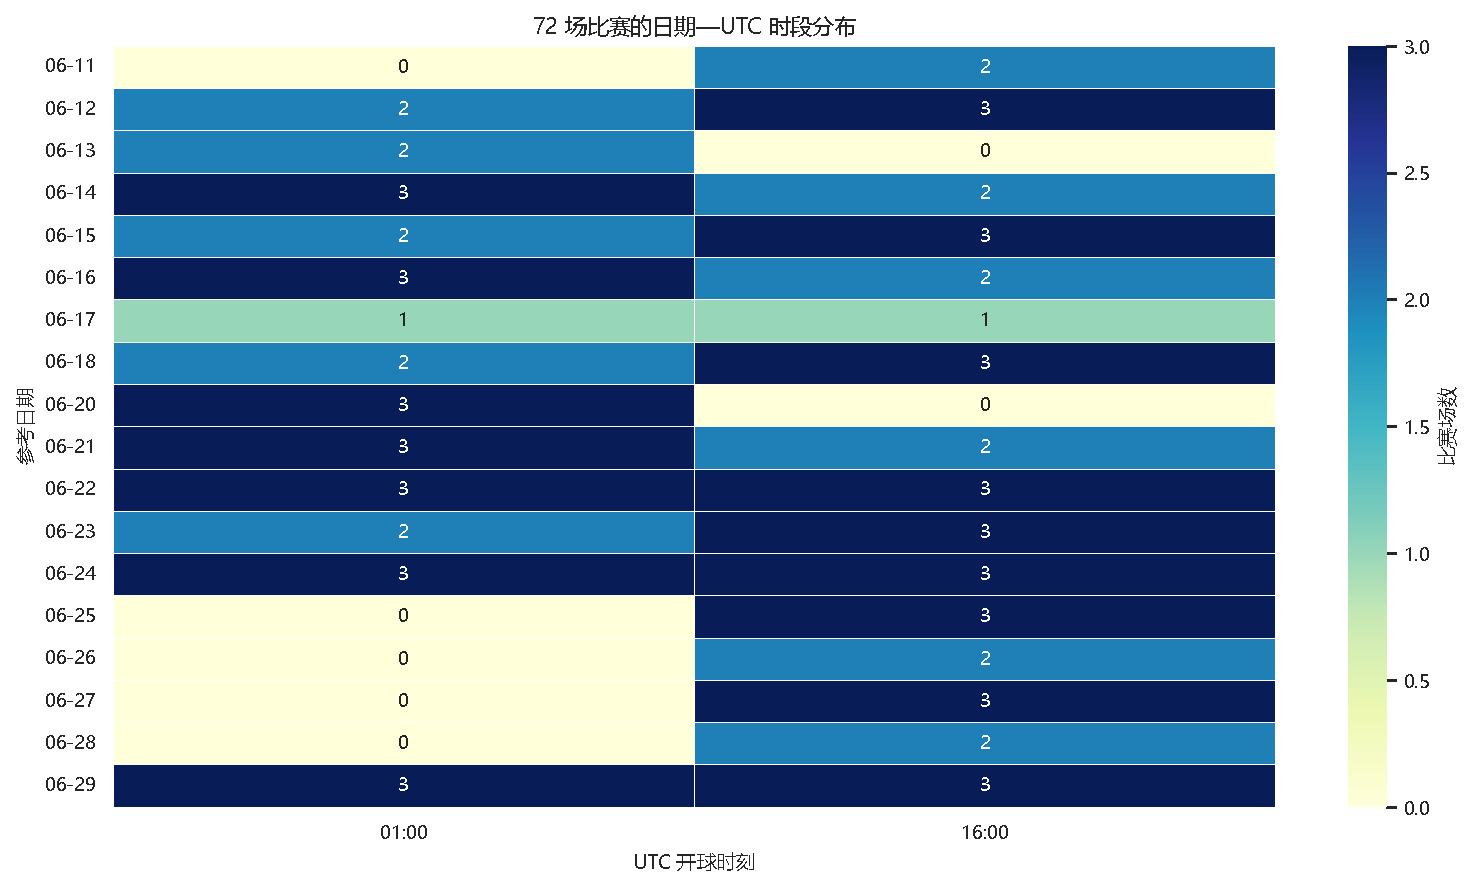
\includegraphics[width=0.94\textwidth]{fig_q2_schedule_heatmap.pdf}
\caption{72 场比赛的日期—UTC 开球时刻热力图。格内数字为该日该 UTC 时刻的比赛数。}
\label{fig:q2-heatmap}
\end{figure}

图~\ref{fig:q2-diagnostics} 将场馆负荷、休息、目标贡献和轮次边界放在同一证据框架中。

场馆负荷同样显示目标与上下限的共同作用。V01--V05 和 V08 达到 8 场上限，V06 承办 6 场，其余 9 个场馆停在 2 场下限。前一类场馆通常在容量、运营成本、气候风险或安保能力的组合上更有利；后一类由每馆最少 2 场的硬约束保留。例如 V04 容量不大，但运营成本较低且气候风险小；V08 则兼具大容量和 4 级安保能力。因此“8 场与 2 场”不是单一容量排序，而是票务、成本、风险和硬下限的取舍。

\begin{figure}[htbp]
\centering
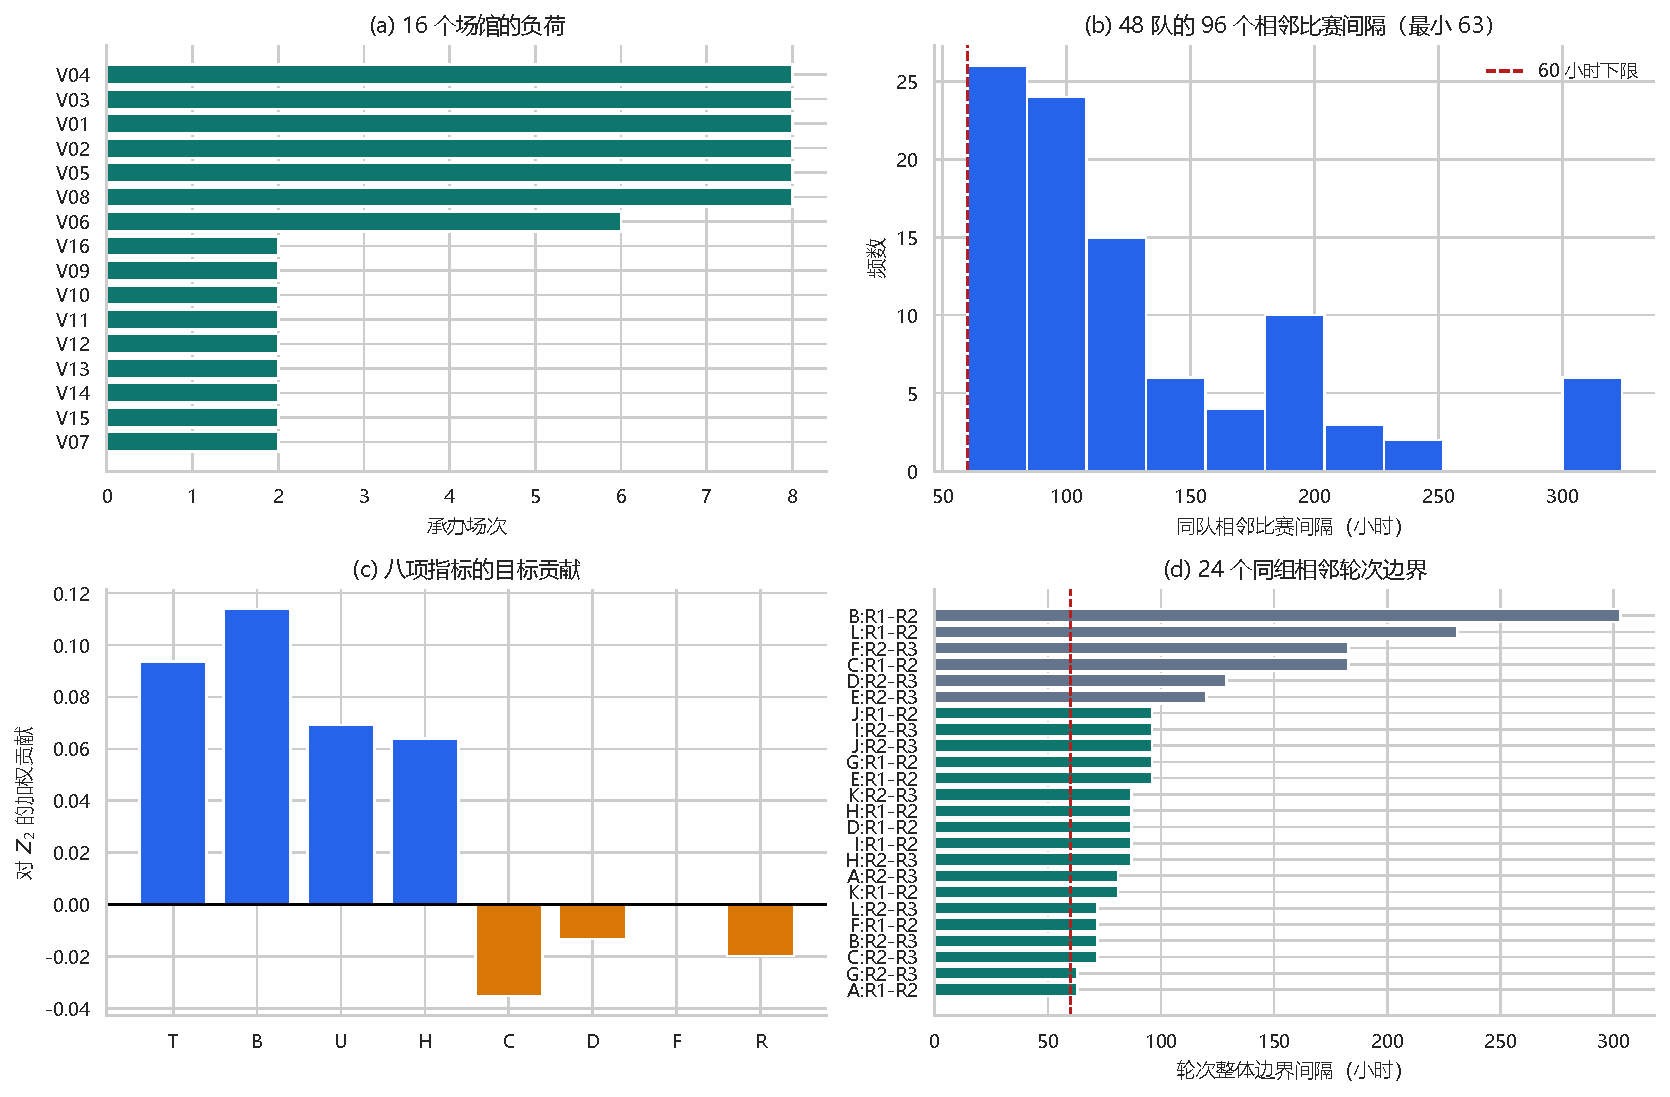
\includegraphics[width=0.98\textwidth]{fig_q2_load_rest_contributions_gaps.pdf}
\caption{问题二的场馆负荷、休息间隔、目标贡献与同组轮次边界。红色虚线为 60 小时下限。}
\label{fig:q2-diagnostics}
\end{figure}

\subsection{权重扰动与近等价排程}

为检查方案是否依赖单一权重组合，保持权重正负方向，分别将 $T,B,C,D,F,R$ 的权重幅值上下扰动 20\%，再将全部权重绝对值归一为 1，每个情景重新求解两个 MILP 并独立复核硬约束。$U,H$ 只由固定对阵决定，在排程中是常数，故不做重求解敏感性。十二个扰动情景全部通过硬约束，$F$ 始终为 0；$D$ 位于 0.187879--0.190562，$R$ 位于 0.403309--0.411664，$C$ 位于 53.015--53.435 百万美元。因此公平、旅行代理、风险和成本的总体结论没有因小范围权重变化而质变。

另一方面，每个情景有 73.6\%--87.5\% 的比赛更换了完整时段--场馆指派。将这些扰动方案统一代回原始权重评价，$Z_2$ 仅在 0.272323--0.272503 之间变化，跨度约 $1.8\times10^{-4}$。这不能直接解释为相应权重对所有决策的因果作用：例如 $T,D,R$ 不进入时段子问题，但时段仍可因大量近等价解和 MIP 容差而改变。故安全的解释是：汇总指标和硬约束较稳定，但具体指派并不唯一，组织者拥有多套近等价的可执行备选。

\begin{figure}[htbp]
\centering
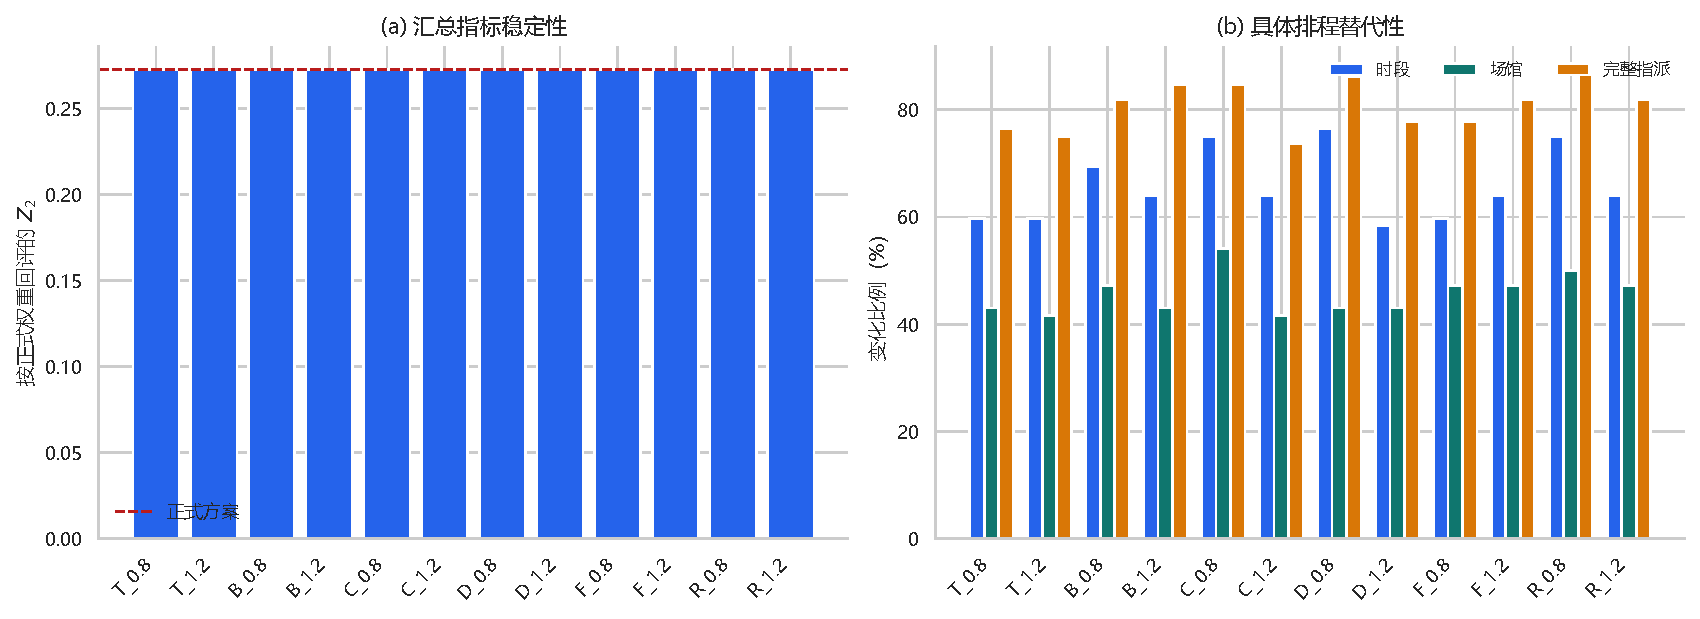
\includegraphics[width=0.94\textwidth]{fig_q2_weight_sensitivity.pdf}
\caption{问题二单项权重±20\% 重求解。左图为各方案在正式原权重下的统一回评；右图分别给出时段、场馆和完整指派的变化比例。}
\label{fig:q2-sensitivity}
\end{figure}

图~\ref{fig:q2-sensitivity} 中大量指派替换与汇总指标的小幅变化共同说明，该问题存在多个指标接近的可行排程。

\FloatBarrier

\section{第三轮动态资源优化}

\subsection{统一信息截面与球队状态}

问题三固定问题二确定的 24 场第三轮比赛、场馆和时段，只调整转播优先级、安保等级、交通保障等级和票价。全部参数在第三轮开始前一次性更新；任一第三轮比赛都不能使用其他第三轮比赛结果。

设球队 \texttt{t} 前两轮已赛场数、积分、累计预期进球、累计预期失球和红牌数分别为 \texttt{G\_t、P\_t、xGF\_t、xGA\_t、RC\_t}。按题面定义状态：

\[
S_t=0.45\frac{P_t}{3G_t}
+0.35\left[0.5+0.5\tanh\left(
\frac{(xGF_t-xGA_t)/G_t}{1.25}
\right)\right]
+0.20\exp\left(-0.55\frac{RC_t}{G_t}\right).
\]

伤病影响 \texttt{h\_t} 取前两轮均值并截断至 0 到 3。第三轮比赛 \texttt{i} 的双方为 \texttt{a、b}，定义：

\[
\Delta_i=0.32(S_a-S_b)-0.055(h_a-h_b).
\]

在赛前基础进球均值上更新：

\[
\lambda_{i,a}=\operatorname{clip}\left(
\lambda_{i,a}^0\exp(\Delta_i-0.04h_a),0.15,4.50
\right),
\]

\[
\lambda_{i,b}=\operatorname{clip}\left(
\lambda_{i,b}^0\exp(-\Delta_i-0.04h_b),0.15,4.50
\right).
\]

\subsection{24 场联合模拟与同分处理}

每次模拟同时从 24 组泊松分布生成第三轮比分\cite{maher1982}，再与前两轮结果合并，统一计算 12 个小组排名和 12 个第三名中的最好 8 队。共模拟 20000 次。球队晋级概率为：

\[
p_t=\frac{1}{20000}\sum_{m=1}^{20000}w_{tm}^{\mathrm{adv}}.
\]

排名只使用积分、净胜球和总进球。当这些指标完全相同且同分区间跨越晋级截止位置时，将剩余名额平均分给同分球队。例如三队完全相同而只剩两个名额，则三队在该次模拟中的晋级权重均为三分之二。该处理同时用于组内前二、第三名身份和最佳第三名第 8 位，不使用球队编号固定破同分。晋级累计矩阵允许浮点权重，每次模拟的晋级权重和严格为 32，20000 次平均晋级概率总和也为 32。

比赛晋级重要性定义为：

\[
Q_i=\frac{4p_a(1-p_a)+4p_b(1-p_b)}{2}.
\]

当双方晋级概率接近 0.5 时，\texttt{Q\_i} 较高；当双方几乎确定晋级或出局时，\texttt{Q\_i} 较低。

\subsection{反馈、需求和吸引力}

前两轮现场和转播反馈先分别计算实际值与赛前预测值之比，对单场比例截断后取球队均值。比赛双方的反馈采用几何平均，记作 \texttt{f\_i\^{}N} 和 \texttt{f\_i\^{}V}。定义：

\[
S_i=\frac{S_a+S_b}{2},\qquad
H_i=\frac{h_a+h_b}{6},\qquad
A_i^0=\frac{\mathrm{attractiveness\_index}_i}{100}.
\]

反馈强度为：

\[
\mathrm{feedback}_i=\operatorname{clip}\left(
\frac{0.5f_i^N+0.5f_i^V-0.75}{0.50},0,1
\right).
\]

更新吸引力为：

\[
A_i=\operatorname{clip}\left[
0.50A_i^0+0.25Q_i+0.12\mathrm{feedback}_i
+0.08S_i+0.05(1-H_i),0,1
\right],
\]

更新现场需求和转播需求为各反馈因子的连乘：

\[
\widetilde N_i=N_i^{\mathrm{pre}}\cdot f_i^N
\cdot(0.88+0.27Q_i)\cdot(0.94+0.12S_i)\cdot(1-0.10H_i),
\]

\[
\widetilde V_i=V_i^{\mathrm{pre}}\cdot f_i^V
\cdot(0.87+0.30Q_i)\cdot(0.90+0.20A_i)\cdot(1-0.06H_i).
\]

\subsection{无激励风险、默契风险和安保风险}

无激励风险为：

\[
R_i^{\mathrm{stake}}=
0.5(2p_a-1)^2+0.5(2p_b-1)^2.
\]

在同一组联合模拟中，分别统计平局、\texttt{a} 胜和 \texttt{b} 胜条件下双方的晋级概率。记：

\[
D_i=\min(p_a^D,p_b^D),
\]

\[
G_i=0.5\max(p_a^W-p_a^D,0)
+0.5\max(p_b^W-p_b^D,0),
\]

则默契风险为：

\[
R_i^{\mathrm{coll}}=\operatorname{clip}\left[
D_i\left(1-\operatorname{clip}(G_i,0,1)\right)
\left(1-0.35R_i^{\mathrm{stake}}\right),0,1
\right].
\]

若某条件样本数为 0，则以该队无条件晋级概率作为保守替代，避免除以 0。动态安保占用率必须使用票价和交通动作之前的更新现场需求：

\[
O_i=\operatorname{clip}\left(\frac{\widetilde N_i}{K_i},0,1\right).
\]

安保需求和综合风险为：

\[
d_i=\operatorname{clip}\left[
0.45d_i^0+0.25O_i+0.15A_i
+0.15\frac{R_i^{\mathrm{stake}}+R_i^{\mathrm{coll}}}{2},0,1
\right],
\]

\[
R_i=0.40R_i^{\mathrm{stake}}
+0.40R_i^{\mathrm{coll}}+0.20d_i m_{q_i}^{R}.
\]

\subsection{资源动作与多重选择 MILP}

每场选择转播优先级 \texttt{b\_i}、安保等级 \texttt{q\_i}、交通等级 \texttt{l\_i} 和票价调整 \texttt{delta\_i}。安保等级不得低于比赛需求，也不得超过场馆能力。对给定交通等级，最终现场需求为：

\[
N_i(\delta_i)=\min\left\{
K_i,\widetilde N_i m_{l_i}^{N}(1+\delta_i)^{\varepsilon_i}
\right\}.
\]

所有票价候选均用容量截断后的完整函数验证：

\[
N_i(\delta_i)\ge 0.88N_i(0).
\]

候选点包括最大折扣、0、最大涨价、需求保持边界和容量切换边界。票务与转播价值为：

\[
TV_i=P_i^0(1+\delta_i)N_i(\delta_i),
\]

\[
\widehat V_i^{\mathrm{upd}}=\widetilde V_i m_{b_i}^{V},\qquad
BV_i=u_i\widehat V_i^{\mathrm{upd}}.
\]

枚举每场合法动作 \texttt{a}，以 \texttt{w\_ia} 表示是否选择该动作。每场恰好选择一个动作，并限制每日高转播、高安保、强化交通和资源预算。为避免与转播观看人数符号冲突，记单场动作的归一化净贡献为

\[
J_{ia}=0.35TV_{ia}'+0.35BV_{ia}'+0.10A_i'
-0.10C_{ia}'-0.10R_{ia}'.
\]

动态目标为：

\[
\max Z_3=\sum_{i\in\mathcal I_3}
\sum_a J_{ia}w_{ia}.
\]

所有标准化边界由第三轮全部更新候选动作统一确定。动态方案的更新边界见表~\ref{tab:q3-bounds}。

\begin{longtable}[]{@{}lrr@{}}
\caption{问题三更新环境的共同归一化边界}\label{tab:q3-bounds}\\
\toprule\noalign{}
指标 & 下界 & 上界 \\
\midrule\noalign{}
\endhead
\bottomrule\noalign{}
\endlastfoot
票务价值 & 2981226.448 & 6558212.829 \\
转播价值 & 4726317.999 & 8519872.166 \\
吸引力 & 0.366896 & 0.686617 \\
资源成本 & 3.000000 & 23.000000 \\
风险 & 0.079917 & 0.745848 \\
\end{longtable}

\subsection{静态方案与动态方案}

静态方案在赛前使用问题二预计现场观众、问题一预计收视、赛前吸引力、赛前无激励风险 \texttt{1-uncertainty\_index} 和默契风险 0，在相同动作集合、每日资源上限和预算下优化。得到的四项动作随后固定。

前两轮结束后，静态方案不得重新选动作，而是在更新环境中按固定的转播、安保、交通和票价重新计算现场需求、票务价值、转播观看人数、转播价值、安保风险、资源成本和净值。动态方案则在更新信息下重新优化。二者最终使用表~\ref{tab:q3-bounds} 的同一更新边界评价。

逐场改善率为：

\[
I_i=\frac{J_i^{\mathrm{dynamic}}-J_i^{\mathrm{static}}}
{|J_i^{\mathrm{static}}|}.
\]

静态净值为 0 时留空。摘要与总体结论使用总净值改善率：

\[
I_{\mathrm{total}}=
\frac{\sum_iJ_i^{\mathrm{dynamic}}-\sum_iJ_i^{\mathrm{static}}}
{\left|\sum_iJ_i^{\mathrm{static}}\right|}.
\]

\subsection{结果与随机种子稳定性}

主种子 20260816 下动态总净值为 6.5838485986，静态总净值为 6.5783676577，因此：

\[
I_{\mathrm{total}}=0.083318\%.
\]

24 场中有 19 场的逐场净值基本不变，4 场正向、1 场负向。动态方案推荐 20 场使用转播优先级 3、4 场使用等级 2；安保等级 1 至 4 的场次数分别为 3、9、10、2；交通等级 1 至 3 的场次数分别为 3、4、17。图~\ref{fig:q3-risk} 表明晋级概率与风险不是单调对应：晋级重要性在概率接近 0.5 时高，而双方已确定晋级时无激励风险反而高。

\begin{figure}[htbp]
\centering
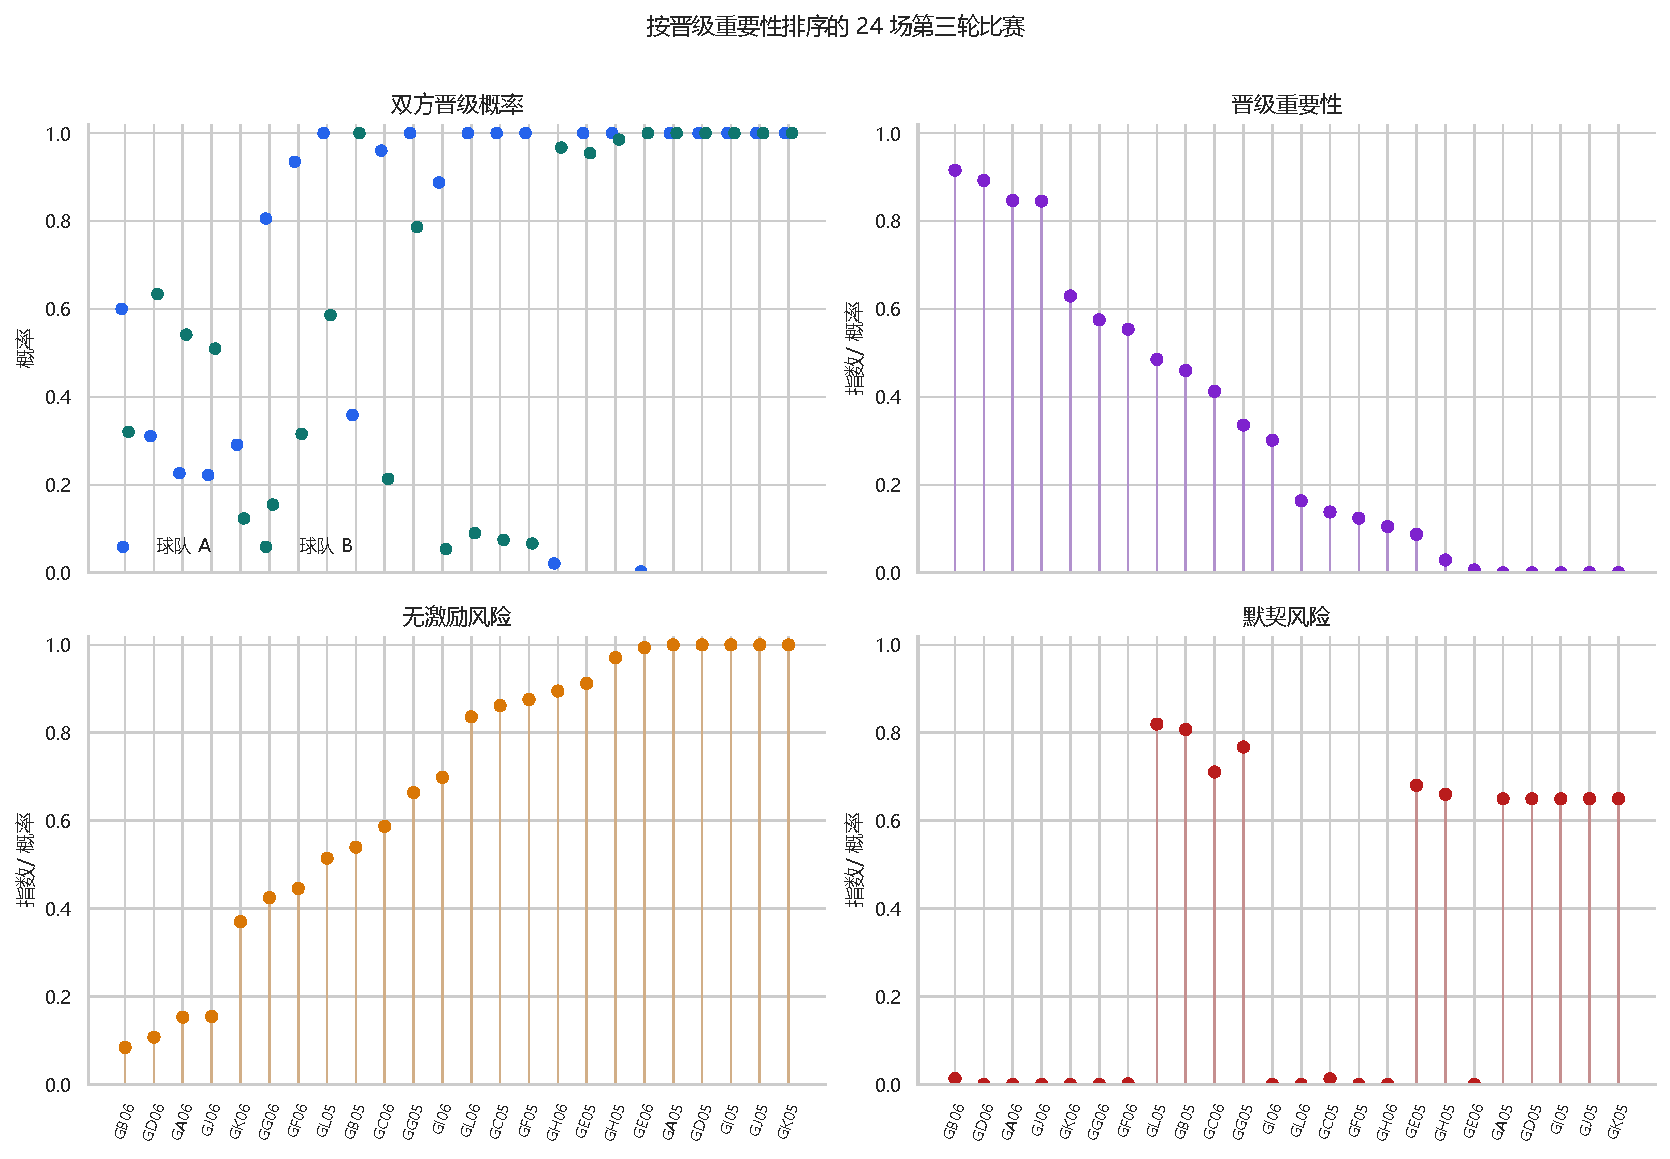
\includegraphics[width=0.98\textwidth]{fig_q3_advancement_and_risk.pdf}
\caption{24 场第三轮比赛的晋级概率、晋级重要性、无激励风险与默契风险。比赛按 $Q_i$ 从高到低排序。}
\label{fig:q3-risk}
\end{figure}

\subsection{五场动作改变的机制}

表~\ref{tab:q3-case-risk}--\ref{tab:q3-case-actions} 只展示非零变化的五场，数据由论文分析脚本从正式输出和更新环境自动重算。动作缩写 \texttt{B/S/T} 依次表示转播、安保和交通等级。

\begin{table}[htbp]
\centering
\caption{五场变化比赛的晋级形势与风险}
\label{tab:q3-case-risk}
\small
\begin{tabular}{lrrrrr}
\toprule
比赛 & A队晋级 & B队晋级 & 重要性 & 无激励 & 默契 \\
\midrule
GA05 & 1.000000 & 1.000000 & 0.000000 & 1.000000 & 0.650000 \\
GF05 & 1.000000 & 0.066587 & 0.124307 & 0.875693 & 0.000207 \\
GG05 & 1.000000 & 0.786392 & 0.335960 & 0.664040 & 0.767586 \\
GJ05 & 1.000000 & 1.000000 & 0.000000 & 1.000000 & 0.650000 \\
GL05 & 1.000000 & 0.585683 & 0.485317 & 0.514683 & 0.819861 \\
\bottomrule
\end{tabular}

\end{table}

\begin{table}[htbp]
\centering
\caption{五场比赛的静态、动态动作与净值}
\label{tab:q3-case-actions}
\scriptsize
\resizebox{\textwidth}{!}{\begin{tabular}{lrrrrr}
\toprule
比赛 & 静态动作 & 动态动作 & 静态净值 & 动态净值 & 改善率 \\
\midrule
GA05 & B3/S2/T3/18.583\% & B2/S2/T2/18.583\% & 0.011215 & 0.000257 & -0.977054 \\
GF05 & B2/S2/T2/18.583\% & B2/S2/T1/18.583\% & 0.048872 & 0.049466 & 0.012167 \\
GG05 & B3/S2/T3/18.583\% & B3/S2/T2/18.583\% & 0.118202 & 0.118265 & 0.000533 \\
GJ05 & B2/S1/T2/18.583\% & B2/S1/T1/18.583\% & -0.073705 & -0.072456 & 0.016943 \\
GL05 & B2/S1/T1/18.583\% & B3/S1/T1/18.583\% & 0.040658 & 0.055190 & 0.357428 \\
\bottomrule
\end{tabular}
}
\end{table}

\texttt{GA05} 的双方晋级概率均为 1，$Q_i=0$，无激励风险和默契风险分别为 1 和 0.65。动态方案将转播由 3 级降至 2 级、交通由 3 级降至 2 级，单场净值由 0.011215 降至 0.000257，是唯一负向变化。这不是求解器错误：多场 MILP 最大化 24 场总净值，并不要求逐场 Pareto 改善。日级高级资源容量存在绑定，但由于本文未计算对偶价格或逐场反事实，不把该资源的唯一受益对象归因于某场比赛。

\texttt{GF05}、\texttt{GG05} 和 \texttt{GJ05} 均将交通等级下调一级，改善率分别为 1.2167\%、0.0533\% 和 1.6943\%；这些场次的更新需求与风险使较高交通等级的边际收益不再覆盖资源成本。\texttt{GL05} 的英格兰和巴拿马晋级概率分别为 1 和 0.585683，$Q_i=0.485317$，且默契风险为 0.819861；动态方案将转播由 2 级提至 3 级，单场净值由 0.040658 增至 0.055190，是五场中绝对改善最大的比赛。

\subsection{日容量、票价边界与模拟收敛}

表~\ref{tab:q3-daily} 中的“用量/容量”显示，6 月 23 日和 29 日的三类高级资源同时达到上限；6 月 24 日和 28 日高转播容量绑定，6 月 20 日高安保容量绑定。预算使用率最高为 86\%，故资源等级数量而非总成本是主要绑定条件。

\begin{table}[htbp]
\centering
\caption{第三轮每日资源使用量与容量}
\label{tab:q3-daily}
\scriptsize
\resizebox{0.92\textwidth}{!}{\begin{tabular}{lrrrr}
\toprule
日期 & 高转播\_用量/容量 & 高安保\_用量/容量 & 强交通\_用量/容量 & 预算使用率\% \\
\midrule
06-20 & 3/4 & 3/3 & 3/4 & 47.500000 \\
06-22 & 1/3 & 1/3 & 1/3 & 19.000000 \\
06-23 & 3/3 & 3/3 & 3/3 & 86.000000 \\
06-24 & 3/3 & 0/2 & 1/3 & 40.000000 \\
06-27 & 3/4 & 1/3 & 3/4 & 42.500000 \\
06-28 & 4/4 & 2/3 & 3/4 & 60.000000 \\
06-29 & 3/3 & 2/2 & 3/3 & 54.000000 \\
\bottomrule
\end{tabular}
}
\end{table}

24 场票价调整均为 18.583183\%。对未触发容量上限的情形，共同弹性 $\varepsilon=-0.75$ 下的 88\% 需求保持边界为

\[
\delta\le 0.88^{1/\varepsilon}-1
=0.88^{-4/3}-1=18.583183\%.
\]

因为 $-1<\varepsilon<0$，未达容量时 $P_i^0(1+\delta)N_i(\delta)\propto(1+\delta)^{1+\varepsilon}$ 随 $\delta$ 增大；达容量后票务价值也随票价上升。程序对每个候选点使用容量截断后的完整 $N_i(\delta)$ 重新验证，因此统一涨幅是共同弹性和需求保持边界的解析结果，并非程序未优化票价。

动态改善较小有三方面原因。其一，静态方案本身已在同一动作集合和日容量下优化，并非最低资源基线；其二，价格弹性和需求保持约束使票价动作高度一致；其三，更新信息只改变少数比赛的边际资源排序，19 场在动态和静态评价中的净值基本相同。因此动态价值主要体现在少量比赛的重新分配，而不是总体资源水平的大幅提高。五随机种子的数值范围见表~\ref{tab:q3-seeds}。

\begin{longtable}[]{@{}lr@{}}
\caption{联合模拟的随机种子稳定性检验}\label{tab:q3-seeds}\\
\toprule\noalign{}
指标 & 五种子范围 \\
\midrule\noalign{}
\endhead
\bottomrule\noalign{}
\endlastfoot
动态总净值 & {[}6.572417, 6.644567{]} \\
静态总净值 & {[}6.566840, 6.639229{]} \\
总体改善率 & {[}0.080406\%, 0.084923\%{]} \\
动态动作与主种子一致率 & 100\% \\
\end{longtable}

五个种子下动作完全一致，且改善率区间较窄，说明结论对 Monte Carlo 随机种子稳定。但该检验不能证明模型对目标权重、泊松独立假设或反馈参数整体稳健。

使用同一主种子，分别用 2000、5000、10000 和 20000 次联合模拟重新建立环境并求解。每个规模都重置随机数生成器，但主客队泊松数组分两次生成，因此这些实验不是严格共用同一随机序列前缀的嵌套收敛检查。表~\ref{tab:q3-convergence} 显示，四种模拟量的 24 场动作与 20000 次基准全部一致，总改善率位于 0.078870\%--0.083318\%。但 2000 次时单队晋级概率最大绝对差仍为 0.027517，5000 次降至 0.007748，10000 次又因随机波动为 0.011833。因此 20000 次对本题的资源动作已足够稳定，但不应声称每支球队的概率估计已严格收敛。

\begin{table}[htbp]
\centering
\caption{主种子下的 Monte Carlo 模拟次数收敛检查}
\label{tab:q3-convergence}
\scriptsize
\resizebox{\textwidth}{!}{\begin{tabular}{lrrrrr}
\toprule
模拟次数 & 晋级概率最大差 & 动作一致率 & 动态总值 & 静态总值 & 总改善率 \\
\midrule
2000 & 0.027517 & 1.000000 & 6.629479 & 6.624254 & 0.000789 \\
5000 & 0.007748 & 1.000000 & 6.621664 & 6.616262 & 0.000816 \\
10000 & 0.011833 & 1.000000 & 6.605048 & 6.599617 & 0.000823 \\
20000 & 0.000000 & 1.000000 & 6.583849 & 6.578368 & 0.000833 \\
\bottomrule
\end{tabular}
}
\end{table}

\begin{figure}[htbp]
\centering
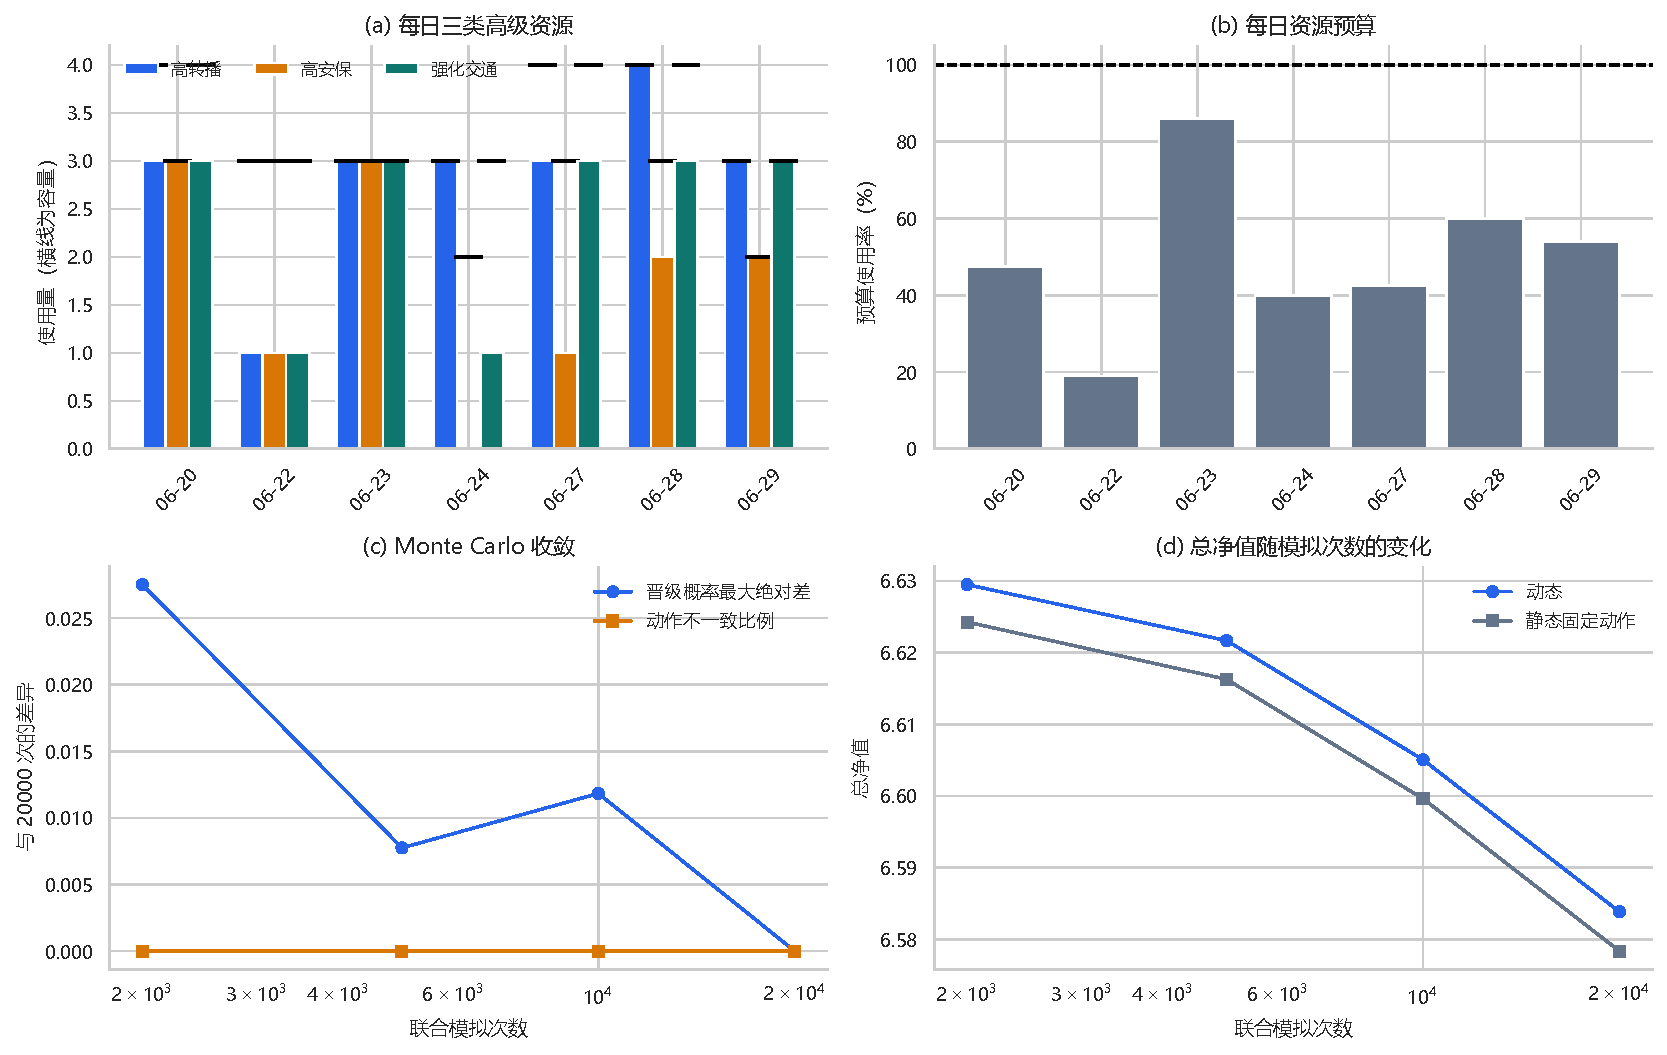
\includegraphics[width=0.80\textwidth]{fig_q3_daily_resources_and_convergence.pdf}
\caption{第三轮每日资源与联合模拟收敛。上左图黑色横线为各日容量；动作不一致比例在四个模拟量下均为 0。}
\label{fig:q3-resources-convergence}
\end{figure}

图~\ref{fig:q3-resources-convergence} 将日资源绑定情况与动作收敛放在同一图中，说明动态调整的主要来源是离散资源数量约束，而非预算耗尽。

\FloatBarrier

\section{与 2022 年世界杯实际赛程比较}

\subsection{数据来源与映射}

实际赛程选取 2022 年卡塔尔世界杯。固定版本 Openfootball JSON 含 64 场比赛，其中小组赛 48 场\cite{openfootball2022}；文件 SHA-256 见支撑材料校验记录。赛前 Elo 表覆盖 32 支球队，无缺失或重复\cite{elo2022}。实体映射统一处理 \texttt{USA} 到 \texttt{United\ States} 等球队别名，并覆盖 8 个实际场馆的城市、容量、经纬度和时区。赛程时间与比分由 FIFA 比赛中心交叉核验\cite{fifa2022}。

模拟赛事有 48 支球队、72 场比赛、16 个场馆和 19 天赛程，2022 年小组赛则有 32 支球队、48 场比赛、8 个场馆和 13 天赛程。总量不能直接作为优劣依据，本文采用三层比较。

\subsection{直接结构事实}

第一层只使用赛程时间和场馆位置直接计算，不借用题目商业参数。旅行按球队赛事内相邻场馆的大圆距离累计，不计首场前往赛区的距离；休息按球队相邻比赛的 UTC 差值计算，结果见表~\ref{tab:q4-structure}。

\begin{table}[htbp]
\centering
\caption{问题四的直接结构事实}\label{tab:q4-structure}
\small
\begin{tabular}{lrr}
\toprule
指标 & 2022 实际赛程 & 优化赛程 \\
\midrule
比赛数 & 48 & 72 \\
球队数 & 32 & 48 \\
场馆数 & 8 & 16 \\
赛程跨度，天 & 13 & 19 \\
每队平均旅行，km & 37.965 & 3715.871 \\
每场平均旅行，km & 25.310 & 2477.247 \\
跨时区转场次数 & 0 & 78 \\
平均休息，h & 97.813 & 128.563 \\
最小休息，h & 87 & 63 \\
休息标准差，h & 5.917 & 63.907 \\
每场馆平均场次 & 6.000 & 4.500 \\
每活跃场馆日平均场次 & 1.021 & 1.043 \\
场馆活跃日利用率 & 0.4519 & 0.2270 \\
\bottomrule
\end{tabular}
\end{table}

优化赛程的平均休息更长，但最小休息更短、休息标准差明显更大，说明 19 天窗口带来的空闲并未均匀分配。2022 年赛程在旅行和跨时区指标上远低于优化赛程，但卡塔尔 8 个场馆集中于单一小范围、没有跨时区，而模拟赛事跨越多个国家和时区。即使换算为每队或每场，地理尺度仍然主导差异，因此不能将较低旅行量完全归因于 2022 排程方法更优。

\subsection{映射辅助指标}

第二层指标需要将实际比赛映射到题目候选对象，但尚未使用完整综合目标。实际 UTC 开球时间按环形小时差映射到同轮次候选时段，以对应时段是否位于 \texttt{global\_prime\_score} 前 20 名判断黄金时段；容量匹配和预计观众使用映射后的题内预计需求，不是 2022 年真实上座数据。

映射辅助指标见表~\ref{tab:q4-auxiliary}。

\begin{longtable}[]{@{}lrr@{}}
\caption{问题四的映射辅助指标}\label{tab:q4-auxiliary}\\
\toprule\noalign{}
指标 & 2022 映射值 & 优化赛程 \\
\midrule\noalign{}
\endhead
\bottomrule\noalign{}
\endlastfoot
黄金时段覆盖率 & 0.666667 & 0.666667 \\
每队平均黄金时段场次 & 2.000 & 2.000 \\
每队黄金时段次数极差 & 3 & 0 \\
容量匹配率 & 0.832326 & 0.601677 \\
题内预计场均观众 & 42051.000 & 41746.417 \\
\end{longtable}

两套赛程的黄金时段覆盖率和队均次数相同，但优化赛程将每队次数极差从 3 降为 0，公平性更好。另一方面，2022 映射容量匹配率更高，题内预计场均观众略高约 304.6 人。这里的``预计观众''来自映射，不可解释为真实 2022 上座人数。

\subsection{完整题内代理评价}

对每场 2022 比赛，先在同轮次题目比赛中按双方赛前 Elo 均值和绝对差寻找最近邻。若实际比赛双方的 Elo 均值和绝对差分别为 $\bar E,\Delta E$，候选比赛为 $\bar E_i,\Delta E_i$，则缩放距离为

\[
d_i^{E}=\frac{|\bar E_i-\bar E|}{200}
+\frac{|\Delta E_i-\Delta E|}{200}.
\]

然后在安保可行后按容量绝对差映射场馆，并按环形 UTC 小时差映射时段。由此借用题内商业、吸引力、安保和风险参数，按问题二的 \texttt{T、B、U、H、C、D、F、R} 定义、边界和权重计算综合值。为降低赛事规模影响，\texttt{T、B、C} 以场均值展示，综合标准化仍使用问题二候选边界。

映射质量是代理结论的前提，而不是可以省略的技术细节。最近邻的 $d_i^E$ 均值和中位数分别为 0.3915 和 0.3550，90\% 分位数为 0.7573；场馆容量差的中位数仅 1100 人，但95\% 分位数达 19972 人，说明少数大场馆难以找到容量接近的题内对象。UTC 小时差的中位数为 0，但90\% 分位数为 6 小时。因此映射并非普遍极远，但存在不可忽略的上尾样本。表~\ref{tab:q4-proxy} 进一步给出统一边界下的完整代理分项。

\begin{longtable}[]{@{}lrrl@{}}
\caption{最近邻映射下的完整题内代理指标}\label{tab:q4-proxy}\\
\toprule\noalign{}
指标 & 2022 实际赛程代理值 & 优化赛程值 & 指标方向 \\
\midrule\noalign{}
\endhead
\bottomrule\noalign{}
\endlastfoot
场均票务价值，USD & 4103559.688 & 3970978.750 & 越大越好 \\
场均转播价值，USD & 4377564.228 & 4535373.132 & 越大越好 \\
悬念均值 & 0.473238 & 0.461436 & 越大越好 \\
吸引力均值 & 0.673815 & 0.639699 & 越大越好 \\
场均成本，百万 USD & 0.718750 & 0.736875 & 越小越好 \\
旅行负担代理 & 0.208229 & 0.189247 & 越小越好 \\
公平性惩罚 & 0.833333 & 0.000000 & 越小越好 \\
执行风险 & 0.483899 & 0.410364 & 越小越好 \\
综合值 & 0.196995 & 0.272453 & 越大越好 \\
\end{longtable}

优化赛程的题内代理综合值较高，主要来自公平性、执行风险、转播价值和旅行负担代理；2022 映射结果在票务、悬念、吸引力和成本上占优。这说明综合分差异不是所有分项同向变化，而是题目权重下的取舍结果。

将最近邻改为排序后的第二近邻，2022 代理综合值由 0.196995 变为 0.210331，仍低于优化赛程的 0.272453，综合方向未反转。由于“第二近邻”本身强制选择排名第二的对象，对象 ID 改变不能解释为自然数据扰动；尤其两种时段映射的小时差分布完全一致，一些 \texttt{slot\_id} 变化只是同一 UTC 小时下的候选 ID 替换。故这项检查只称为局部映射敏感性。

为检查综合方向是否由某一组权重巧合造成，用固定种子 20260816 对八项权重幅值独立乘以 $\mathrm U(0.8,1.2)$，保持正负方向并重新归一化，共生成 2000 组固定赛程的回评权重。最近邻下 $Z_2^{\mathrm{opt}}-Z_2^{2022}$ 位于 0.05602--0.09722，第二近邻下位于 0.04677--0.07941；两组各 2000 次均未反转。这一结论仅支持：在固定赛程、固定映射、固定指标和小范围权重扰动下，题内代理综合方向保持不变；它不是重新排程后的全模型稳健性，也不是对映射假设、Elo 数据源或真实世界杯价值的全面证明。

\noindent 图~\ref{fig:q4-three-layer} 对应前述三层口径，图~\ref{fig:q4-mapping} 解释映射距离与代理分差的来源，图~\ref{fig:q4-weights} 则显示权重扰动下的方向边界。

\begin{figure}[htbp]
\centering
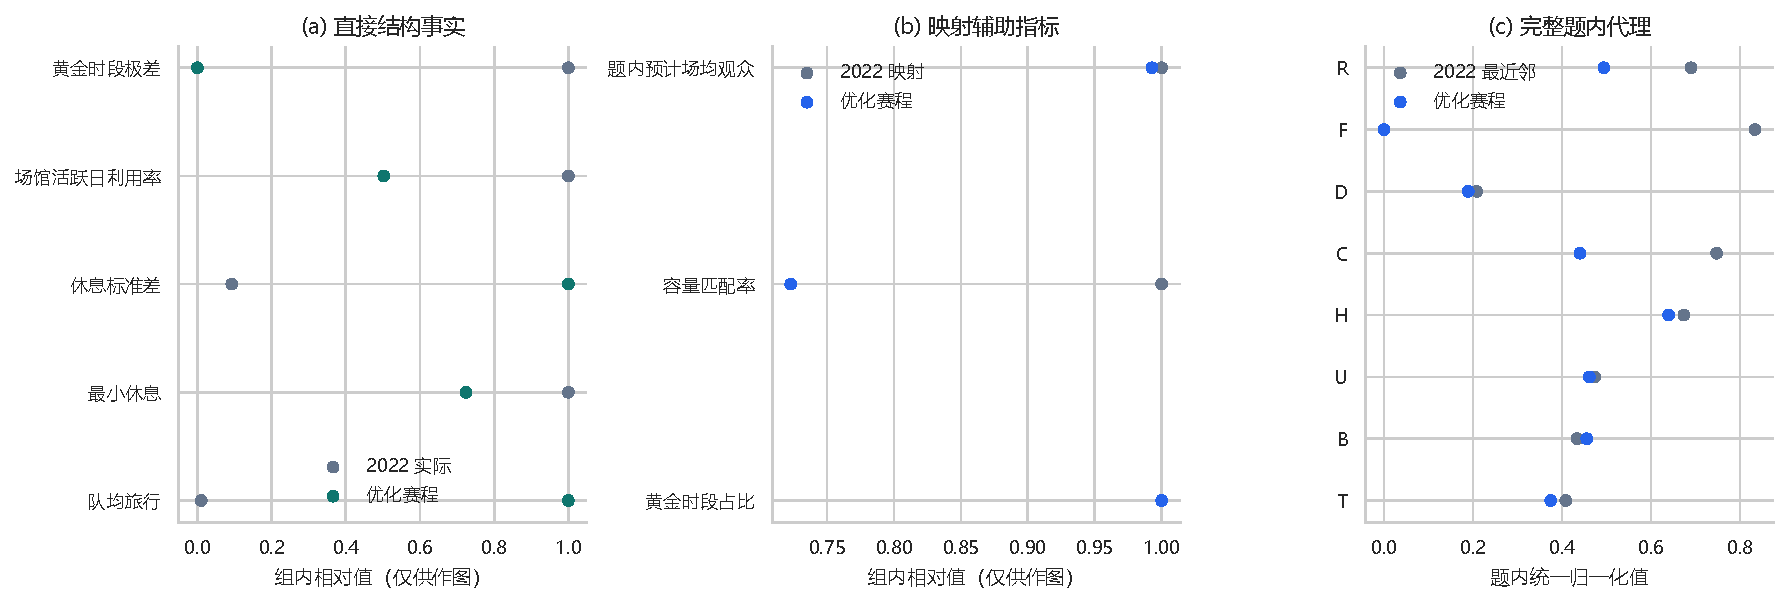
\includegraphics[width=0.98\textwidth]{fig_q4_three_layer_comparison.pdf}
\caption{问题四的三层比较。前两个分图为解决量纲差异而对每对数值按该对最大值缩放，只比较同一指标内的相对位置。}
\label{fig:q4-three-layer}
\end{figure}

\begin{figure}[htbp]
\centering
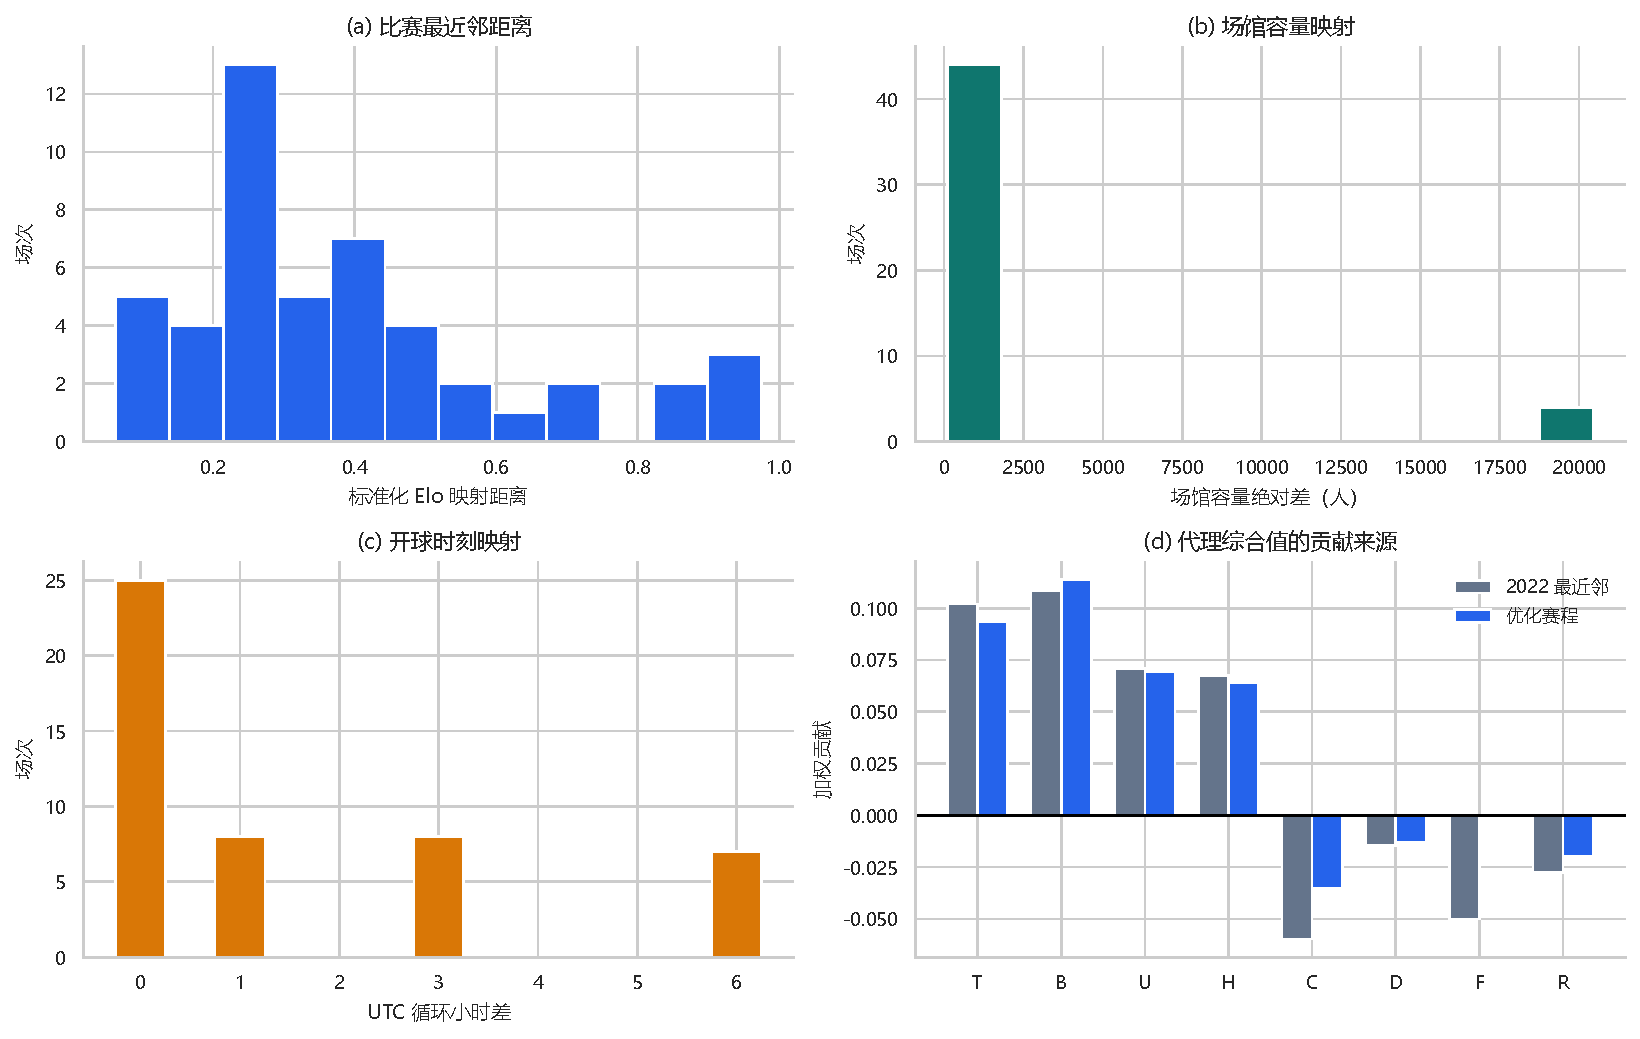
\includegraphics[width=0.98\textwidth]{fig_q4_mapping_quality_and_contributions.pdf}
\caption{最近邻映射质量与代理综合值的分项贡献。容量差存在少数近 2 万人的上尾映射。}
\label{fig:q4-mapping}
\end{figure}

\begin{figure}[htbp]
\centering
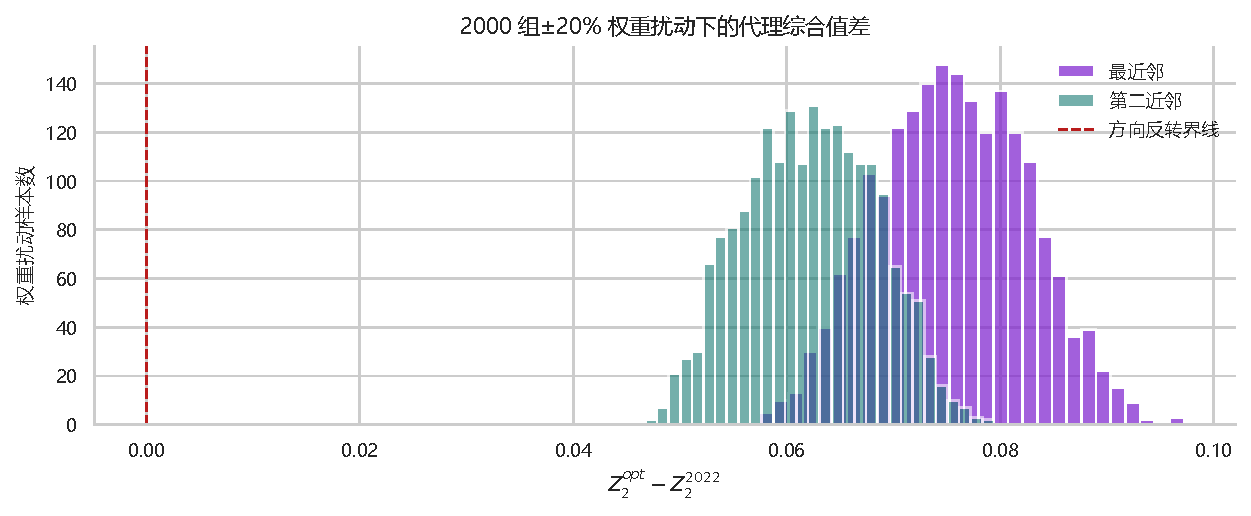
\includegraphics[width=0.82\textwidth]{fig_q4_weight_sensitivity.pdf}
\caption{2000 组±20\% 权重扰动下的代理综合值差分布。零点左侧表示综合方向反转。}
\label{fig:q4-weights}
\end{figure}

\FloatBarrier

\section{模型评价与局限}

\subsection{模型特点}

本文首先用统一信息时点连接四问，使问题一预测、问题二排程和问题三更新之间不存在未来信息倒流。问题一的对称特征保证球队记录顺序不影响预测，时间扩窗验证比随机划分更接近真实外推。问题二将全部硬约束转化为可独立复算的 UTC、场馆和资源条件，并报告标准化边界和目标贡献。问题三按题面同时模拟 24 场，使用浮点晋级权重处理完全同分，并把静态动作固定后置于同一更新环境评价。问题四没有将代理指标伪装为真实经营数据，而是把直接事实、映射辅助量和完整代理量分层解释。

\subsection{局限性}

问题一的 Elastic Net 不能充分表示复杂非线性，也无法吸收临赛新闻等附件外信息。对数逆变换直接使用 \texttt{expm1}，没有额外估计对数正态偏差修正；时间外残差也显示极端热门与冷门场次存在向中心收缩。因此 72 场预测更适合用作附件信息口径下的相对转播需求，不能替代临赛实时修正。

问题二采用时段与场馆分解，不能证明三维联合模型全局最优。旅行负担又是上一轮全部安保合格候选场馆下的均值代理，没有用转移变量描述实际连续路线；部分小组出现较长轮次空档，表明目标中缺少对过度空闲的直接惩罚。

问题三的泊松模型假定给定状态后进球独立，未描述比赛中红牌、领先后的战术变化和双方进球相关性。五种子检验只覆盖 Monte Carlo 随机性；约 0.083\% 的改善较小，其实际管理价值还取决于题目资源成本指数与真实成本的对应程度。

问题四的 2022 比较受赛事规模和举办区域影响。卡塔尔的紧凑地理条件天然降低旅行和时区成本；完整代理层还依赖 Elo 最近邻、场馆容量和时段映射，无法覆盖转播合同、球队基地、城市治理、政治和实际安保安排。

\section{结论}

问题一以对称赛前特征和对数目标建立收视预测模型。Elastic Net 在扩窗验证中的 MSE 为 188.978683，优于 Extra Trees 和均值基线；统一特征函数将世界杯同义赛事名称归一，测试集和未来 72 场的未见赛事类别数均为 0。72 场预测均值为 161.599758 百万人，其高于训练拟合均值的主要原因是世界杯赛事指示量的正向贡献。

问题二采用时段 MILP 与固定时段后的场馆 MILP 分解求解，得到 \texttt{Z\_2=0.272453} 的可行排程。两个子问题均在设定 MIP 容差内求得最优解，但不据此声明三维联合模型的最优性。最终每队获得 2 场黄金时段和 1 场大容量场馆比赛，公平性惩罚为 0，球队及同组轮次最小间隔均为 63 小时，全部硬约束复算通过。

问题三在第三轮开始前的统一信息截面上进行 20000 次 24 场联合泊松模拟，完全同分时采用等比例晋级权重。静态固定方案和动态方案在同一更新边界下的总净值分别为 6.578368 和 6.583849，总体改善率为 0.083318\%。变化集中 4 场正向、1 场负向，负向场次体现了联合资源优化允许单场牺牲的取舍。五个随机种子与四种模拟次数下动作选择一致，说明这一小幅边际改善对 Monte Carlo 设置稳定，但不构成对其他模型假设的全面稳健性证明。

问题四显示，优化赛程在题内代理口径下的综合值高于 2022 实际赛程的两种邻近映射结果，且黄金时段分配更均衡；但 2022 赛程在最小休息、休息波动、场馆活跃日利用率、旅行和容量匹配等方面表现更好或更紧凑。旅行差异主要受到举办区域尺度影响，因此合理结论是两套赛程在不同组织条件下呈现指标取舍，而不是本文方案对真实世界杯安排的全面替代。


\section*{AI 工具使用声明}
\addcontentsline{toc}{section}{AI 工具使用声明}
本参赛队在竞赛过程中使用了 AI 工具，主要用于建模方案讨论、程序调试、结果复核与语言表达整理，详细使用情况见支撑材料。

\begingroup
\raggedright
\sloppy
\begin{thebibliography}{99}
\bibitem{problem2026} 2026年度“策联杯”数学建模精英联赛 C 题及数据附件，2026。
\bibitem{zou2005} Zou H, Hastie T. Regularization and Variable Selection via the Elastic Net. \textit{Journal of the Royal Statistical Society: Series B}, 2005, 67(2): 301--320.
\bibitem{geurts2006} Geurts P, Ernst D, Wehenkel L. Extremely Randomized Trees. \textit{Machine Learning}, 2006, 63: 3--42.
\bibitem{maher1982} Maher M J. Modelling Association Football Scores. \textit{Statistica Neerlandica}, 1982, 36(3): 109--118.
\bibitem{huangfu2018} Huangfu Q, Hall J A J. Parallelizing the Dual Revised Simplex Method. \textit{Mathematical Programming Computation}, 2018, 10: 119--142.
\bibitem{scipymilp} SciPy Developers. \texttt{scipy.optimize.milp}---SciPy Reference Guide. \url{https://docs.scipy.org/doc/scipy/reference/generated/scipy.optimize.milp.html}, accessed 2026-08-16.
\bibitem{highs} HiGHS Development Team. HiGHS: High-performance software for linear optimization. \url{https://highs.dev/}, accessed 2026-08-16.
\bibitem{openfootball2022} Openfootball. World Cup 2022 JSON, commit 516d3825c3bd23fdc298c4014e84bde78f2d4965. \url{https://github.com/openfootball/worldcup.json/blob/516d3825c3bd23fdc298c4014e84bde78f2d4965/2022/worldcup.json}.
\bibitem{fifa2022} FIFA. FIFA World Cup Qatar 2022 Match Centre. \url{https://www.fifa.com/tournaments/mens/worldcup/qatar2022/match-center}.
\bibitem{elo2022} International Football. World Football Elo Ratings Table, 2022-11-12. \url{https://www.international-football.net/elo-ratings-table?confed=&day=12&month=11&old-team=&year=2022}.
\end{thebibliography}
\endgroup

\typeout{MAIN-TEXT-END-PAGE=\thepage}
\clearpage
\appendix
\section{支撑材料文件列表}

支撑材料与论文采用相同的最终计算版本，主要文件如下：
\begin{enumerate}[leftmargin=3em]
  \item \texttt{code/run\_all.py}：四问计算流水线入口；
  \item \texttt{code/pipeline\_core.py}：特征、预测、MILP、联合模拟和比较指标；
  \item \texttt{code/check\_outputs.py}：公式、约束、输出和可复现性验收；
  \item \texttt{code/paper\_analysis.py}：论文专用的扩窗、系数、敏感性、收敛与映射质量分析；
  \item \texttt{requirements.txt}：固定 Python 依赖版本；
  \item \texttt{requirements-paper.txt}：论文作图与 PDF 质检的附加依赖；
  \item \texttt{output/}：四问最终 CSV 与 \texttt{diagnostics.json}；
  \item \texttt{paper/generated/}：由论文分析脚本自动生成的图、表和可追溯结果；
  \item \texttt{material/user\_data/worldcup\_2022\_openfootball.json}：2022 年赛程原始数据；
  \item \texttt{material/user\_data/worldcup\_2022\_pre\_tournament\_elo.csv}：2022 年赛前 Elo；
  \item \texttt{material/user\_data/entity\_mappings.json}：球队与场馆实体映射；
  \item \texttt{AI 工具使用详情.pdf}：AI 工具、用途、交互与人工核验说明。
\end{enumerate}

\section{复现命令与算法摘要}

完整源程序作为独立支撑材料提交，不在论文附录重复排印。在项目根目录执行：

\begin{lstlisting}[language=bash,numbers=none]
python -m venv .venv
source .venv/bin/activate
python -m pip install -r requirements.txt
python code/run_all.py --output-dir output
python code/check_outputs.py --output-dir output
python code/paper_analysis.py --output-dir output --generated-dir paper/generated
\end{lstlisting}

问题一使用单一特征函数完成赛事名称规范化、对称特征构造、时间扩窗与全量重训练。问题二先解时段 MILP，再在时段固定后解场馆 MILP；问题三先生成 20000 次联合比分并计算浮点晋级权重，再枚举合法动作并解多重选择 MILP。问题四在固定实体映射上计算结构层与题内代理层指标。

\section{输出校验摘要}

自动验收重新训练问题一并逐值比对预测，复算问题二的全部指标、UTC 容量、同组轮次边界和场馆约束，验证问题三晋级权重总和、票价边界、静态动作固定复算和五种子结果，并检查问题四的三份来源材料、赛程结构与 30 项比较指标。正式结果的最终状态为 \texttt{CHECK PASSED}。

\section{完整源程序}

根据论文格式规范第三条，附录给出全部完整、可运行源程序；附录页数不计入正文 30 页限制。

\subsection{流水线入口}
\lstinputlisting[language=Python]{../code/run_all.py}

\subsection{模型与计算核心}
\lstinputlisting[language=Python]{../code/pipeline_core.py}

\subsection{自动验收程序}
\lstinputlisting[language=Python]{../code/check_outputs.py}

\subsection{论文分析与作图程序}
\lstinputlisting[language=Python]{../code/paper_analysis.py}

\end{document}
